\documentclass[12pt]{report}
\usepackage{graphicx}
\usepackage{color}
\usepackage{longtable}
\usepackage{amsmath}
\usepackage{hyperref}
\usepackage{comment}
\usepackage{xspace}
\usepackage{array}
\usepackage{authblk}

\setlength\oddsidemargin{-5mm}
\setlength\topmargin{-2.0cm}
\setlength\evensidemargin{-5mm}
\setlength\textwidth{170mm}
\setlength\textheight{240mm}
\setlength\parindent{0mm}
\setlength\parskip{5mm}

\def\species{\mathrm{sp}}
\def\phase{\mathrm{ph}}
\def\massfrac{\chi}
\def\flux{\mathbf{F}}
\def\darcyvel{\mathbf{v}}
\def\energydens{\mathcal{E}}
\def\d{\mathrm{d}}
\def\diag{\mathrm{diag}\,}

\newcommand{\uo}{\mbox{UO\textsubscript{2}}\xspace}
\DeclareMathOperator{\erfc}{erfc}

\begin{document}

\title{MOOSE's PorousFlow module:\\verification tests}

\author{Andy Wilkins}
\author{Chris Green}
\affil{CSIRO}

\maketitle

\abstract{This document describes the physics captured by MOOSE's
  PorousFlow module, as well as describing various numerical aspects
  and tips to ensure good convergence.

Each nontrivial test in the test suite {\em has its own separate
  documentation} and these should help users understand more clearly
how to build a PorousFlow input file.

Within this document, black text indicates funcionality that has been
implemented and tested \textcolor{red}{and red text indicates
  functionality that should be implemented by December 2017}.  }

\tableofcontents

\documentclass[]{scrreprt}
\usepackage{amsmath,amsfonts,graphicx}
\usepackage{multirow}
\usepackage{pslatex}
\usepackage{tabularx}
\usepackage{comment}
\usepackage{xspace}
\usepackage{array}

\usepackage{hyperref}

\usepackage{caption}
\DeclareCaptionFont{white}{\color{white}}
\DeclareCaptionFormat{listing}{\colorbox{gray}{\parbox{\textwidth}{#1#2#3}}}

\graphicspath{
{figures/}
}

\def\species{\mathrm{sp}}
\def\phase{\mathrm{ph}}
\def\massfrac{\chi}
\def\flux{\mathbf{F}}
\def\darcyvel{\mathbf{v}}
\def\energydens{\mathcal{E}}
\def\d{\mathrm{d}}

\newcommand{\uo}{\mbox{UO\textsubscript{2}}\xspace}

\setcounter{secnumdepth}{3}


\begin{document}


\title{Mass-Conservation Tests}
\author{CSIRO}
\maketitle

\tableofcontents

\chapter{PorousFlowComponentMass postprocessor}

\section{Single-phase, single-component}
\label{1phase1comp.sec}

The total fluid mass of species $\species$ within a volume $V$ is
\begin{equation}
\int_{V} \phi\sum_{\phase}\rho_{\phase} S_{\phase}\massfrac_{\phase}^{\species} \ .
\end{equation}
It must be checked that MOOSE calculates this correctly in order that
mass-balances be correct, and also because this quantity is used in a
number of other tests

A 1D model with $-1\leq x \leq 1$, and with three elements of size 1 is
created with the following properties:
\begin{center}
\begin{tabular}{|ll|}
\hline
Constant fluid bulk modulus & 1\,Pa \\
Fluid density at zero pressure & 1\,kg.m$^{-3}$ \\
Van Genuchten $m$ & 0.5 \\
Van Genuchten $\alpha$ & 1\,Pa$^{-1}$ \\
Porosity & 0.1 \\
\hline
\end{tabular}
\end{center}
The porepressure is set at $P=x$.

Recall that in PorousFlow, mass is lumped to the nodes.  Therefore,
the integral above is evaluated at the nodes, and a sum of the results
is outputted as the PorousFlowComponentMass postprocessor.
Using the properties given above, this yields:
\begin{center}
\begin{tabular}{|ccccc|}
\hline
$x$ & $p$ & Density & Saturation & Nodal mass \\
\hline
-1 & -1 & 0.367879441 & 0.707106781 & 0.008671002 \\
-0.333333333 & -0.333333333 & 0.716531311 & 0.948683298 & 0.02265871 \\
-0.333333333 & -0.333333333 & 0.716531311 & 0.948683298 & 0.02265871 \\
0.333333333 & 0.333333333 & 1.395612425 & 1 & 0.046520414 \\
0.333333333 & 0.333333333 & 1.395612425 & 1 & 0.046520414 \\
1& 1 & 2.718281828 & 1 & 0.090609394 \\
\hline
 & & & Total & 0.237638643 \\
\hline
\end{tabular}
\end{center}
MOOSE also gives the total mass as 0.237638643\,kg.  This test is part of
the automatic test suite that is run every time the code is updated.

\newpage

\section{Single-phase, two-components}

The same test as Section~\ref{1phase1comp.sec} is run but with two
components.  The mass fraction is fixed at
\begin{equation}
\massfrac_{\phase=0}^{\species=0} = x^{2} \ .
\end{equation}

\begin{center}
\begin{tabular}{|ccccccc|}
\hline
$x$ & $p$ & Density & Saturation & $\massfrac_{\phase=0}^{\species=0}$
& Nodal mass$_{\species=0}$ & Nodal mass$_{\species=1}$ \\
\hline
-1 & -1 & 0.367879441 & 0.707106781 & 1 & 0.008671 & 0 \\
-0.333333333 & -0.333333333 & 0.716531311 & 0.948683298 & 0.111111 &
0.00251763 & 0.02014108 \\
-0.333333333 & -0.333333333 & 0.716531311 & 0.948683298 & 0.111111 &
0.00251763 & 0.02014108 \\
0.333333333 & 0.333333333 & 1.395612425 & 1 & 0.111111 & 0.00516893 &
0.04135148 \\
0.333333333 & 0.333333333 & 1.395612425 & 1 & 0.111111 & 0.00516893 &
0.04135148 \\
1& 1 & 2.718281828 & 1 & 1 & 0.09060939 & 0 \\
\hline
 & & & & Total & 0.11465353 & 0.12298511 \\
\hline
\end{tabular}
\end{center}

MOOSE produces the expected answer.

\newpage

\section{Two-phase, two-components}

This test computes the mass for two components in two phases, with both components present in
both phases. The mass fractions are fixed at
\begin{equation}
\massfrac_{\phase=0}^{\species=0} = 0.3 \ , \massfrac_{\phase=1}^{\species=0} = 0.55 .
\end{equation}

Pressure is fixed at 1 Pa for each phase, and density is given by a constant bulk modulus fluid with denisty
at zero pressure given by 1 kg m$^{-3}$ and 0.1 kg m$^{-3}$ for phase 0 and phase 1, respectively, giving densities of $2.7128$
kg m$^{-3}$ for phase 0, and $0.27128$ kg m$^{-3}$ for phase 1. Saturation of phase 0 varies linearly
with $x$ throughout the 1D model with three elements from $ 0 \le x \le 1$

For component species 0, the mass at each node is calculated as
\begin{center}
\begin{tabular}{|ccccccc|}
\hline
$x$ & $S_{\phase=0}$ & $\massfrac_{\phase=0}^{\species=0}$ & $\massfrac_{\phase=1}^{\species=0}$
& Nodal mass$_{\phase=0}^{\species=0}$ & Nodal mass$_{\phase=1}^{\species=0}$ & Total nodal mass$^{\species=0}$ \\
\hline
0 & 0 & 0.3 & 0.55 & 0 & 0.00249176 & 0.00249176 \\
0.33333 & 0.33333 & 0.3 & 0.55 & 0.00453047 & 0.00166117 & 0.00619164 \\
0.33333 & 0.33333 & 0.3 & 0.55 & 0.00453047 & 0.00166117 & 0.00619164 \\
0.66667 & 0.66667 & 0.3 & 0.55 & 0.00906094 & 0.000830586 & 0.009891526 \\
0.66667 & 0.66667 & 0.3 & 0.55 & 0.00906094 & 0.000830586 & 0.009891526 \\
1 & 1 & 0.3 & 0.55 & 0.0135914 & 0 & 0.0135914 \\
\hline
 & & & Total & 0.0407742 & 0.0074753 & 0.0482495 \\
\hline
\end{tabular}
\end{center}

For component species 1, the mass at each node is calculated as
\begin{center}
\begin{tabular}{|ccccccc|}
\hline
$x$ & $S_{\phase=0}$ & $\massfrac_{\phase=0}^{\species=0}$ & $\massfrac_{\phase=1}^{\species=0}$
& Nodal mass$_{\phase=0}^{\species=0}$ & Nodal mass$_{\phase=1}^{\species=0}$ & Total nodal mass$^{\species=0}$ \\
\hline
0 & 0 & 0.7 & 0.45 & 0 & 0.00203871 & 0.00203871 \\
0.33333 & 0.33333 & 0.7 & 0.45 & 0.01057110 & 0.001359141& 0.01193024\\
0.33333 & 0.33333 & 0.7 & 0.45 & 0.01057110 & 0.001359141 & 0.01193024 \\
0.66667 & 0.66667 & 0.7 & 0.45 & 0.02114219 & 0.000679570 & 0.02182176 \\
0.66667 & 0.66667 & 0.7 & 0.45 & 0.02114219 & 0.000679570 & 0.02182176 \\
1 & 1 & 0.7 & 0.45 & 0.03171329 & 0 & 0.03171329 \\
\hline
 & & & Total & 0.0951399 & 0.06116113 & 0.1012560 \\
\hline
\end{tabular}
\end{center}

MOOSE produces the expected answer.


\end{document}

\chapter{Jacobian Tests}

\section{Fluid-mass time derivative}

The following tests of the Jacobian are performed on the fluid-mass time derivative kernel (PorousFlowMassTimeDerivative).
\begin{enumerate}
\item single-phase, with a single component, with a van-Genuchten capillary pressure, constant bulk-modulus density and constant porosity.
\item single-phase, with 3 components, with a van-Genuchten capillary pressure, constant bulk-modulus density and constant porosity.
\item 2-phase PP formulation, with 2 components (that exist in both phases), with a van-Genuchten capillary pressure, constant bulk-modulus density for each phase and constant porosity.
\item 2-phase PP formulation, with 3 components (that exist in both phases), with a van-Genuchten capillary pressure, constant bulk-modulus density for each phase and constant porosity.
\end{enumerate}


\section{Fluid Advective Flux}

The following tests of the Jacobian are performed on the fluid-mass advective flux kernel (PorousFlowAdvectiveFlux).
\begin{enumerate}
\item single-phase, with 1 component, constant viscosity, constant insitu-permeability, density with constant bulk modulus, Corey relative permeability, nonzero gravity, with van-Genuchten capillary pressure.
\item single-phase, with 3 components, constant viscosity, constant insitu-permeability, density with constant bulk modulus, Corey relative permeability, nonzero gravity, with van-Genuchten capillary pressure.
\item 2-phase (PP formulation), with 2 components (that exist in both phases), constant viscosity for each phase, constant insitu-permeability, density with constant bulk modulus for each phase, Corey relative permeability for each phase, nonzero gravity, with van-Genuchten capillary pressure.
\item 2-phase (PP formulation), with 3 components (that exist in both phases), constant viscosity for each phase, constant insitu-permeability, density with constant bulk modulus for each phase, Corey relative permeability for each phase, nonzero gravity, with van-Genuchten capillary pressure.
\end{enumerate}

\chapter{Dirac kernels}
\section{Geometric tests}

The test suite contains tests that demonstrate:
\begin{itemize}
\item when a point sink is placed at a node, it withdraws fluid (or heat) from only that node;
\item when a point sink that is proportional to mobility (or relative
  permeability, etc) is placed in an element where some nodes have
  zero mobility (or relative permeability, etc), then fluid (or heat)
  is not extracted from those nodes.
\end{itemize}

\section{Peaceman borehole fluxes}

The automatic test suite contains four tests that check that the Peaceman flux
\begin{equation}
f(P_{i}, x_{i}) =
W \left|C(P_{i}-P_{\mathrm{bh}})\right|
\frac{k_{\mathrm{r}}\rho}{\mu}(P_{i} - P_{\mathrm{bh}})
\label{bh.propto.eqn}
\end{equation}
is correctly implemented.  A vertical borehole is placed through the
centre of a single element, and fluid flow to the borehole as a
function of porepressure is measured.  The tests are
\begin{itemize}
\item A production borehole with $P_{\mathrm{bh}} = 0$, with a
  fully-saturated medium.
\item An injection borehole with $P_{\mathrm{bh}} = 10$\,MPa, with a
  fully-saturated medium.
\item A production borehole with $P_{\mathrm{bh}} = -1$\,MPa, with an
  unsaturated medium.
\item An injection borehole with $P_{\mathrm{bh}} = 0$, with an
  unsaturated medium.
\end{itemize}
The parameters common to these tests are:
\begin{center}
\begin{tabular}{|ll|}
\hline
Element size & $2\times 2\times 2$\,m$^{3}$ \\
Borehole radius & 0.1\,m \\
Permeability & $10^{-12}$\,m$^{2}$ \\
Gravity & 0 \\
Unit fluid weight & 0 \\
Fluid reference density & 1000\,kg.m$^{-3}$ \\
Fluid bulk modulus & 2\,GPa \\
Fluid viscosity & $10^{-3}$\,Pa.s \\
Van Genuchten $\alpha$ & $10^{-5}$\,Pa \\
Van Genuchten $m$ & 0.8  \\
Residual saturation & 0 \\
FLAC relperm $m$ & 2 \\
\hline
\end{tabular} \\
\end{center}
It is remotely possible that the MOOSE implementation {\em applies}
the borehole flux incorrectly, but {\em records} it as a Postprocessor
correctly as specified by Eqn~(\ref{bh.propto.eqn}).  Therefore, these
four simulations also record the fluid mass and mass-balance error in
order to check that the fluid mass is indeed being correctly changed
by the borehole.  Figure~\ref{bh02_05.fig} demonstrates that
Eqn~(\ref{bh.propto.eqn}) is indeed correctly implemented in MOOSE.

\begin{figure}[htb]
\centering
\begin{tabular}{cc}
\includegraphics[width=7cm]{bh02_flow.pdf} &
\includegraphics[width=7cm]{bh02_error.pdf} \\
\includegraphics[width=7cm]{bh03_flow.pdf} &
\includegraphics[width=7cm]{bh03_error.pdf} \\
\includegraphics[width=7cm]{bh04_flow.pdf} &
\includegraphics[width=7cm]{bh04_error.pdf} \\
\includegraphics[width=7cm]{bh05_flow.pdf} &
\includegraphics[width=7cm]{bh05_error.pdf} \\
\end{tabular}
\caption{Left figures: Comparison between the MOOSE result (in dots), and the
  expected behaviour of the borehole flux given by
  Eqn~(\ref{bh.propto.eqn}) (as a line) for the cases listed in the
  text.  Right
  figures: The mass balances, which are all small.}
\label{bh02_05.fig}
\end{figure}

\section{Comparison with analytic solution}
The Richards' equation for a fully-saturated medium with $\rho \propto
\exp(P/B)$ and large constant bulk modulus $B$ becomes Darcy's equation
\begin{equation}
\frac{\partial}{\partial t}\rho =  \nabla_{i}\alpha_{ij}\nabla_{j}\rho
\end{equation}
where $\alpha_{ij} = k_{ij}B/(\mu\phi)$, with notation described
in the Theory Manual.   In the isotropic case (where $k_{ij} =
\kappa \delta_{ij}$), the steadystate equation is just Laplace's
equation
\begin{equation}
\nabla^{2}\rho = 0 \ ,
\end{equation}
Place a borehole of radius $r_{\mathrm{bh}}$ and infinite length
oriented along the $z$ axis.  Then the situation becomes 2D and can be
solved in cylindrical coordinates, with $\rho=\rho(r,\theta)$ and
independent of $z$.  If the pressure at the borehole wall
$r=r_{\mathrm{bh}}$ is $P_{\mathrm{bh}}$, then the fluid density is
$\rho_{\mathrm{bh}} \propto \exp(P_{\mathrm{bh}}/B)$.  Assume that at
$r=R$ the fluid pressure is held fixed at $P_{R}$, or equivalently the
density is held fixed at $\rho_{R}$.  Then the solution of Laplace's
equation is well-known to be
\begin{equation}
\rho = \rho_{\mathrm{bh}} + (\rho_{R} - \rho_{\mathrm{bh}})
\frac{\log(r/r_{\mathrm{bh}})}{\log(R/r_{\mathrm{bh}})} \ .
\label{eqn.log.bh}
\end{equation}
This is the fundamental solution used by Peaceman and others to derive
expressions for $W$ by comparing with numerical expressions resulting
from Eqn~(\ref{bh.propto.eqn}) (see Theory Manual for more details).

Chen and Zhang (see Theory manual) have derived an expression for $W$
in the case where this borehole is placed at a node in a square mesh.
This test compares the MOOSE steadystate solution with a single
borehole with $W$ defined by
Chen and Zhang's formula is compared with Eqn~(\ref{eqn.log.bh}) to
illustrate that the MOOSE implementation of a borehole is correct.

Figure~\ref{bh07.fig} shows this comparison.  Most parameters in this
study are identical to those given in the above table with the
following exceptions: the mesh is shown in Fig~\ref{bh07.mesh.fig};
the permeability is $10^{-11}$\,m$^{2}$; the borehole radius is 1\,m;
the borehole pressure is $P_{\mathrm{bh}}=0$; the outer radius is
$r=300$\,m; and the outer pressure is $P_{R}=10$\,MPa.

\begin{figure}[htb]
\centering
\includegraphics[width=8cm]{bh07_mesh.pdf}
\caption{The mesh used in the comparison with Eqn~(\ref{eqn.log.bh}),
  with the green dot indicating the position of the borehole.
  The central elements are $10\times 10$\,m$^{2}$, and the outer
  boundary is at $r=300$\,m.}
\label{bh07.mesh.fig}
\end{figure}

\begin{figure}[htb]
\centering
\includegraphics[width=12cm]{bh07.pdf}
\caption{Comparison of the MOOSE results (dots) with the analytical
  solution Eqn~(\ref{eqn.log.bh}) for the steadystate porepressure
  distribution surrounding single borehole.}
\label{bh07.fig}
\end{figure}

\chapter{PorousFlow sink boundary conditions}

A number of different sink boundary conditions have been implemented
in PorousFlow.  (To make these into sources instead of sinks, the
strength of the flux just needs to be made negative.)  All the sinks
are implemented using full upwinding.  This is to prevent the sink
from attempting to remove fluid from a node that actually contains no
fluid.

The basic sink uses a Function to specify the flux on the boundary,
and also has the option of multiplying by any combination of: the
fluid mobility, the relative permeability, or a mass fraction.  These
latter multiplying factors are all useful in the case of sinks to
prevent an unlimited amount of fluid being withdrawn from the porous
medium, which can lead to extremely poor nonlinear convergence even if
only one node in the entire mesh is ``running dry''.

Derived from the basic one, is another boundary condition that allows
the flux to be modified by a piecewise-linear function of
porepressure, which is useful for the case where transfer coefficients
are defined across the boundary, or more complicated situations.

Also derived from the basic one are two others, in which the flux is
governed by a half Gaussian or half cubic function of porepressure,
which are useful for modelling evapotranspiration through a boundary.

\section{Basic sink}
\label{basic.sec}

\subsection{Test 1}

A sink flux of strength 6\,kg.m$^{-2}$.s$^{-1}$ is applied to the left
edge ($x=0$) of a 3D mesh.  A single-phase, single-component fluid is
used, and the porepressure is initialised to $p=y+1$ (for $0\leq y\leq
1$).  No fluid flow within the element is used, so the masses of fluid
at the finite-element nodes behave independently.  The fluid is
assumed to have density $\rho = 1.1 \exp(p/1.3)$ [kg.m$^{-3}$].  The
porosity is 0.1.

Under these conditions, assuming $p\geq 0$ so that the porous medium
is fully saturated with fluid, the fluid mass at a node should obey
\begin{equation}
m = V\phi\rho = V\times0.1\times 1.1\exp(p/1.3) = m(t=0) - 6At \ ,
\end{equation}
where $V$ is the volume occupied by the node, and $A$ is its area
exposed to the flux.  MOOSE correctly produces this result, as
illustrated in Figure~\ref{s01.fig}.

\begin{figure}[htb]
\begin{center}
\includegraphics[width=8cm]{s01.pdf}
\caption{Results of Test 1, illustrating that MOOSE correctly applies
  a constant sink flux to boundary nodes.}
\label{s01.fig}
\end{center}
\end{figure}

\subsection{Test 2}

An identical setup to Test 1 is used here, but with the sink flux
strength being multiplied by the mobility:
\begin{equation}
\mbox{mobility} = n_{i}k_{ij}n_{j}\rho/\nu \ ,
\end{equation}
where $n_{i}k_{ij}n_{j}$ is the permeability tensor $k$ projected onto
the normal direction to the boundary $n$, and the fluid density and
viscosity are $\rho$ and $\nu$, respectively.  In this example
$\nu=1.1$\,Pa.s and $n_{i}k_{ij}n_{j}=0.2$\,m$^{2}$.  The other
parameters are the same as Test 1, except now the strength of the flux
is 6\,Pa.s$^{-1}$.

In this case, the expected result is (for $p>0$)
\begin{equation}
\frac{\d m}{\d t} = V\phi \frac{\d \rho}{\d t} = -6 A
\frac{n_{i}k_{ij}n_{j}\rho}{\mu} \ .
\end{equation}
MOOSE correctly produces this result, as illustrated in
Figure~\ref{s02.fig}.

\begin{figure}[htb]
\begin{center}
\includegraphics[width=8cm]{s02.pdf}
\caption{Results of Test 2, illustrating that MOOSE correctly applies
  a constant sink flux modified by the fluid mobility.  (A slight
  drift away from the expected result is due to MOOSE taking large
  time steps.)}
\label{s02.fig}
\end{center}
\end{figure}


\subsection{Test 3}

An identical setup to Test 1 is used here, but with the sink flux
strength being multiplied by the relative permeability, which is
chosen to be:
\begin{equation}
\kappa_{\mathrm{rel}} = S^{2} \ ,
\end{equation}
with $S$ being the fluid saturation.  A van-Genuchten capillary
relationship is used:
\begin{equation}
S = \left( 1 + (-\alpha p)^{1/(1-m)} \right)^{-m} \ ,
\end{equation}
with $\alpha = 1.1$\,Pa$^{-1}$, and $m=0.5$.  The porepressure is
initialised to be $p=-y$.  The other parameters are
identical to Test 1.

In this case, the expected result is
\begin{equation}
\frac{\d m}{\d t} = V\phi \frac{\d \rho S}{\d t} = -6 A S^{2} \ .
\end{equation}
MOOSE correctly produces this result, as illustrated in
Figure~\ref{s03.fig}.

\begin{figure}[htb]
\begin{center}
\includegraphics[width=8cm]{s03.pdf}
\caption{Results of Test 3, illustrating that MOOSE correctly applies
  a constant sink flux modified by the fluid relative permeability.}
\label{s03.fig}
\end{center}
\end{figure}


\subsection{Test 4}

A similar setup to Test 1 is used here, but with a 3-component,
single-phase fluid, with the sink flux only extracting the second
component, with a rate proportional to the mass fraction of that
component.  This test checks that the flux is correctly implemented
(see Figure~\ref{s07.fig}) and that the correct fluid component is being
withdrawn from the correct nodes.  MOOSE produces the expected result.

\begin{figure}[htb]
\begin{center}
\includegraphics[width=8cm]{s07.pdf}
\caption{Results of Test 4, illustrating that MOOSE correctly applies
  a sink flux of a particular fluid component proportional to the
  component's mass fraction.}
\label{s07.fig}
\end{center}
\end{figure}


\subsection{Test 5}

A sink is applied to the left edge ($x=0$) of a 3D mesh.  A
3-component, 2-phase fluid is used.  Call the two phases ``water'' and
``gas''.  The porepressures are initialised to $p_{\mathrm{water}} =
y$ and $p_{\mathrm{gas}} = y + 3$.  The mass fractions are initialised
to $(0.3, 0.35, 0.35)$ in the water phase, and $(0.1, 0.8, 0.1)$ in
the gas phase.  The water phase is assumed to have density
$\rho_{\mathrm{water}} = 1.5 \exp(p_{\mathrm{water}}/2.3)$, and the gas phase
$\rho_{\mathrm{gas}} = 1.1 \exp(p_{\mathrm{gas}}/1.3)$.  A van-Genuchten capillary
relationship is used:
\begin{equation}
S_{\mathrm{water}} = \left( 1 + (\alpha (p_{\mathrm{gas}} - p_{\mathrm{water}})^{1/(1-m)} \right)^{-m} \ ,
\end{equation}
with $\alpha = 1.1$\,Pa$^{-1}$, and $m=0.5$.  The water relative
permeaility is assumed to be Corey type with exponent $1$, and the gas
phase has exponent $2$ (that is $\kappa_{\mathrm{rel,gas}} =
S_{\mathrm{gas}}^{2}$, with $S_{\mathrm{gas}} = 1 -
S_{\mathrm{water}}$).

The sink flux acts only on the second component.  It is multiplied by the
relative permeability of the gas phase, and the mass fraction of the
second component in the gas phase.  This is possibly meaningless
physically, but acts as a good test of the PorousFlowSink.  In this
test the mass fractions remain fixed: there is nothing to induce a
change of a component from the water phase to the gas phase since the
only Kernels used are mass-conservation Kernels that simply demand
mass conservation of each fluid component (summed over each phase).

The test checks whether MOOSE is correctly applying the sink flux, and
that the fluid-component masses at the nodes respond correctly to the
flux.  Figure~\ref{s08.fig} demonstrates that MOOSE produces the
expected result.

\begin{figure}[htb]
\begin{center}
\includegraphics[width=8cm]{s08.pdf}
\caption{Results of Test 5, illustrating that in a 2-phase system
  MOOSE correctly applies a sink flux of a particular fluid component
  proportional to the component's mass fraction and the relative
  permeaility of the gas phase.}
\label{s08.fig}
\end{center}
\end{figure}



\section{Piecewise-linear sink}
\label{piecewise.sec}

A sink flux of strength
\begin{equation}
f = \left\{
\begin{array}{ll}
8 & \mbox{ if } p > 0.8 \\
8(p + 0.2) & \mbox{ if } 0.3 \leq p \leq 0.8 \\
4 & \mbox{ if } p < 0.3 \ ,
\end{array}
\right.
\end{equation}
(measured in kg.m$^{-2}$.s$^{-1}$) is applied to the right side
($x=1$) of a 3D mesh.  A single-phase, single-component fluid is used,
and the porepressure is initialised to $p=y+1$ (for $0\leq y \leq 1$).
No fluid flow within the element is used, so the masses of fluid at
the finite-element nodes behave independently.  The fluid is assumed
to have density $\rho = 1.1 \exp(p/1.3)$ [kg.m$^{-3}$].  The porosity
is 0.1.

Under these conditions, the expected result for the fluid mass at a
node on the right side of the mesh is
\begin{equation}
\frac{\d m}{\d t} = V\phi \frac{\d \rho S}{\d t} = -f A \ .
\end{equation}
The notation is the same as in previous sections.

The test checks that the mass evolves according to this equation, and
that the flux is applied correctly.  Figure~\ref{s04.fig} demonstrates
agreement with the expected flux and the MOOSE implementation.

\begin{figure}[htb]
\begin{center}
\includegraphics[width=8cm]{s04.pdf}
\caption{A piecewise-linear sink flux is correctly modelled by MOOSE}
\label{s04.fig}
\end{center}
\end{figure}



\section{Half-Gaussian sink}
\label{half_gaussian.sec}

A sink flux of strength
\begin{equation}
f = \left\{
\begin{array}{ll}
6 & \mbox{ if } p \geq 0.9 \\
6\exp\left(-\frac{1}{2} \left(\frac{p-0.9}{0.5} \right)^{2}\right) & \mbox { if } p < 0.9 \ .
\end{array}
\right.
\end{equation}
(measured in kg.m$^{-2}$.s$^{-1}$) is applied to the right side
($x=1$) of a 3D mesh.  This is a half-Gaussian sink with center
0.9\,Pa, standard deviation 0.5\,Pa and maximum 6.  A single-phase,
single-component fluid is used, and the porepressure is initialised to
$p=y+1.4$ (for $0\leq y \leq 1$).  No fluid flow within the element is
used, so the masses of fluid at the finite-element nodes behave
independently.  The fluid is assumed to have density $\rho = 1.1
\exp(p/1.3)$ [kg.m$^{-3}$].  The porosity is 0.1.  A van-Genuchten capillary
relationship is used:
\begin{equation}
S = \left( 1 + (-\alpha p)^{1/(1-m)} \right)^{-m} \ ,
\end{equation}
with $\alpha = 1.1$\,Pa$^{-1}$, and $m=0.5$.

Under these conditions, the expected result for the fluid mass at a
node on the right side of the mesh is
\begin{equation}
\frac{\d m}{\d t} = V\phi \frac{\d \rho S}{\d t} = -f A \ .
\end{equation}
The notation is the same as in previous sections.

The test checks that the mass evolves according to this equation, and
that the flux is applied correctly.  Figure~\ref{s05.fig} demonstrates
agreement with the expected flux and the MOOSE implementation.

\begin{figure}[htb]
\begin{center}
\includegraphics[width=8cm]{s05.pdf}
\caption{A half-Gaussian sink flux with center 0.9\,Pa and standard
  deviation 0.5\,Pa is correctly modelled by MOOSE}
\label{s05.fig}
\end{center}
\end{figure}



\section{Half-cubic sink}
\label{half_cubic.sec}

A sink flux of strength
\begin{equation}
f = \left\{
\begin{array}{ll}
3 & \mbox{ if } p \geq 0.9 \\
\frac{3}{(-0.8)^3} (2(p-0.9) + 0.8) (p - 0.9 + 0.8)^2 & \mbox{ if }
0.1 < p < 0.9 \\
0 & \mbox{ if } p \leq 0.1
\end{array}
\right.
\end{equation}
(measured in kg.m$^{-2}$.s$^{-1}$) is applied to the right side
($x=1$) of a 3D mesh.  This is a half-cubic sink with center
0.9\,Pa, cutoff $-0.8$\,Pa, and maximum 3\,kg.m$^{-2}$.s$^{-1}$.  A
single-phase, single-component fluid is used, and the porepressure is
initialised to $p=x(y+1)$ (for $0\leq y \leq 1$ and $0\leq x \leq 1$).
No fluid flow within the element is used, so the masses of fluid at
the finite-element nodes behave independently.  The fluid is assumed
to have density $\rho = 1.1 \exp(p/1.3)$ [kg.m$^{-3}$].  The porosity
is 0.1.

Under these conditions, the expected result for the fluid mass at a
node on the right side of the mesh is
\begin{equation}
\frac{\d m}{\d t} = V\phi \frac{\d \rho S}{\d t} = -f A \ .
\end{equation}
The notation is the same as in previous sections.

The test checks that the mass evolves according to this equation, and
that the flux is applied correctly.  Figure~\ref{s06.fig} demonstrates
agreement with the expected flux and the MOOSE implementation.

\begin{figure}[htb]
\begin{center}
\includegraphics[width=8cm]{s06.pdf}
\caption{A half-cubic sink with center 0.9\,Pa, cutoff $-0.8$\,Pa, and
  maximum 3\,kg.m$^{-2}$.s$^{-1}$ is correctly modelled by MOOSE.}
\label{s06.fig}
\end{center}
\end{figure}


\chapter{Advection of a fluid component}

The porepressure at a boundary may be maintained at a fixed value by
applying a sufficiently strong piecewise-linear sink:
\begin{equation}
f = Cp \ ,
\end{equation}
(measured in kg.m$^{-2}$.s$^{-1}$) for large\footnote{If $C$ is too
  large then it will dominate the numerics and MOOSE will not
  converge.} conductance $C$.  In the multi-component case, the flux
of of fluid component $\kappa$ should be made proportional to the
component mass fraction, $\chi^{\kappa}$:
\begin{equation}
f^{\kappa} = C\chi^{\kappa}p \ .
\label{eqn.flux.rhs}
\end{equation}
This is a ``natural'' boundary condition, in that fluid exits or
enters the porous material at a rate dictated by the mass-fraction
within the porous material.  This means, for instance, that if fluid
is exiting ($p>0$ in this case) then only components that exist at the
boundary system will exit, and MOOSE will not attempt to extract fluid
components that have zero mass-fraction.

This example concerns a 1D porous material occupying the space $0\leq
x \leq 1$.  It contains a single phase fluid with two
fluid components.  The porous material initially only contains fluid
component $1$, and there is a pressure gradient:
\begin{equation}
p(t=0) = 1 - x \ \ \ \mbox{and}\ \ \ \chi^{0}(t=0) = 0 \ .
\end{equation}
For $t>0$, fluid component $0$ is introduced on the material's left
side ($x=0$), by applying the fixed boundary conditions:
\begin{equation}
p(x=0) = 1 \ \ \ \mbox{and}\ \ \ \chi^{0}(x=0) = 1 \ .
\end{equation}
The right-hand side, at $x=1$, is subjected to the flux of
Eqn~(\ref{eqn.flux.rhs}).  The fluid-component $0$ flows from the left
side to the right side via the pressure gradient.  To simplify the
following analysis, the fluid bulk modulus is taken to be very large.

Because the fluid bulk modulus is very large, $\partial P/\partial x = -1$ is a
solution for all time.  This means that the governing equation reduces
to
\begin{equation}
\phi \frac{\partial \chi}{\partial t} =  (k_{ij}/\mu) \nabla_{j}
\chi \nabla_{i}P \ .
\end{equation}
In this equation $\phi$ is the porosity, $k_{ij}$ is the permeability
tensor, and $\mu$ is the fluid viscosity.  This is just the advection
equation for the mass fraction $\chi$, with velocity
\begin{equation}
\mbox{velocity}_{j} = \nabla_{i}P\frac{k_{ij}}{\mu\phi} \ .
\end{equation}
In this test, the parameters are chosen such that velocity$=1$\,m.s$^{-1}$.

The sharp front (described by the advection equation
with the initial and boundary conditions) is {\em not} maintained by
MOOSE.  This is due to numerical diffusion, which is particularly
strong in the upwinding scheme implemented in the PorousFlow module.
Nevertheless, MOOSE advects the smooth front with the correct
velocity, as shown in Figure~\ref{s09.fig}.

The sharp front is {\em not} maintained by MOOSE even when no
upwinding is used.  In the case at hand, which uses a fully-saturated
single-phase fluid, the {\tt FullySaturated} versions of the Kernels
may be used in order to compare with the standard fully-upwinded
Kernels.  The {\tt FullySaturated} Kernels do not employ any upwinding
whatsoever, so less numerical
diffusion is expected.  This is demonstrated in
Figure~\ref{s09.fig}.  Two additional points may also be
nocied: (1) the lack of upwinding has produced a ``bump'' in the
mass-fraction profile near the concentrated side; (2) the lack of upwinding
means the temperature profile moves slightly slower than it should.
These two affects reduce as the mesh density is increased, however.

\begin{figure}[htb]
\begin{center}
\begin{tabular}{cc}
\includegraphics[width=7cm]{s09_0_1.pdf}  &
\includegraphics[width=7cm]{s09_0_5.pdf}
\end{tabular} \\
\includegraphics[width=7cm]{s09_1_0.pdf}
\caption{Results of the advection of a fluid component test,
  illustrating that the numerical implementation of porous flow within
  MOOSE diffuses sharp fronts, but advects them at the correct
  velocity ($v=1$\,m.s$^{-1}$ in this case, and notice the centre of
  the front is at the correct position in each picture).  Less
  diffusion is experienced when upwinding is not used.  Top left: mass
  fraction at $t=0.1$\,s.  Top right: mass fraction at $t=0.5$\,s.
  Bottom: mass fraction at $t=1.0$\,s.}
\label{s09.fig}
\end{center}
\end{figure}

\documentclass[]{scrreprt}
\usepackage{amsmath,amsfonts,graphicx}
\usepackage{multirow}
\usepackage{pslatex}
\usepackage{tabularx}
\usepackage{comment}
\usepackage{xspace}
\usepackage{array}

\usepackage{hyperref}

\usepackage{caption}
\DeclareCaptionFont{white}{\color{white}}
\DeclareCaptionFormat{listing}{\colorbox{gray}{\parbox{\textwidth}{#1#2#3}}}

\graphicspath{
{figures/}
}

\def\species{\mathrm{sp}}
\def\phase{\mathrm{ph}}
\def\massfrac{\chi}
\def\flux{\mathbf{F}}
\def\darcyvel{\mathbf{v}}
\def\energydens{\mathcal{E}}
\def\d{\mathrm{d}}

\newcommand{\uo}{\mbox{UO\textsubscript{2}}\xspace}

\setcounter{secnumdepth}{3}


\begin{document}


\title{Gravity-Head Tests}
\author{CSIRO}
\maketitle

\tableofcontents

\chapter{Establishment of gravity head in 1D}

These tests concern the steadystate pressure distribution obtained
either by running a transient model for a long time, or by running a
steady-state analysis, both of which should lead to the same result.
Without fluxes, the steadystate pressure distribution is just
\begin{equation}
P(x) = P_{0} - \rho_{0} g x \ ,
\end{equation}
if the fluid bulk modulus, $B$, is large enough compared with $P$.
Here $P_{0}$ is the porepressure at $x=0$.  For smaller bulk modulus
\begin{equation}
P(x) = -B \log\left( e^{-P_{0}/B} + \frac{g\rho_{0}x}{B} \right) \ .
\label{grav.head.eqn}
\end{equation}
Here it is assumed that the density is given by $\rho = \rho_{0}e^{-P/B}$
with constant bulk modulus, $g$ is the
magnitude acceleration due to gravity (a vector assumed to be pointing in the
negative $x$ direction), and $x$ is position.  The tests described below
are simple tests and are part of the automatic test suite.

\section{Single-phase, single-component}
\label{1phase1comp.sec}

Two single-phase simulations with 100 1D elements are run: one with
fully-saturated conditions, and the other with unsaturated conditions
using the van-Genuchten capillary pressure (this should not, and does
not, make any difference to the results).  The porepressure is held
fixed at one boundary ($x=0$).

An example verification is shown in Figure~\ref{gh.fig}, which also
shows results from a 2-phase simulation (see Section~\ref{2phase.sec}).

\begin{figure}[htb]
\centering
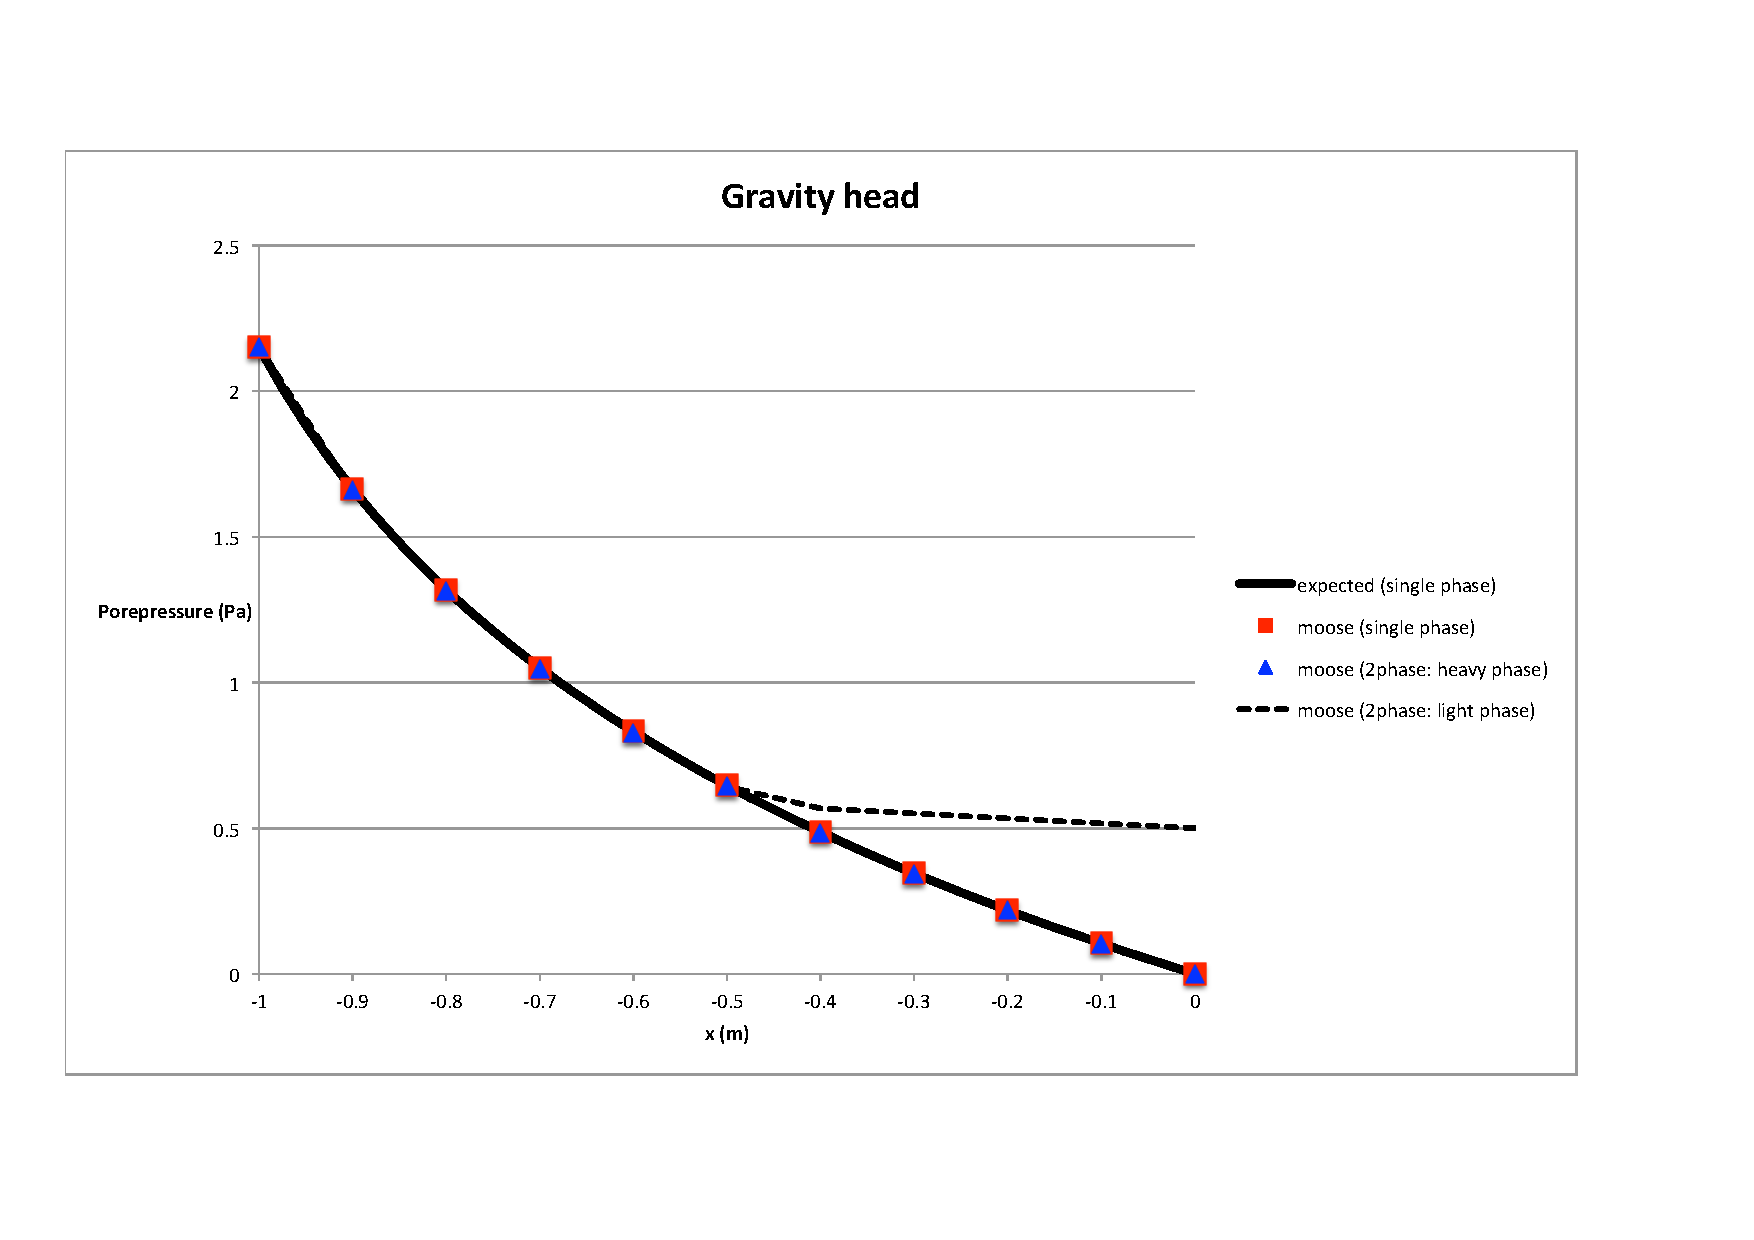
\includegraphics[width=15cm]{gravity_fig.pdf}
\caption{Comparison between the MOOSE result (in dots), and the
  exact analytic expression given by Eqn~(\ref{grav.head.eqn}).
  test had 10 elements in the $x$ direction, with $-1\leq x \leq
  0$\,m.  The parameters were $B=1.2$\,Pa, $\rho_{0}=1$\,kg.m$^{-3}$,
  and $g=-1$\,m.s$^{-2}$.  For the two-phase simulation, the light
  phase had $B=1$\,Pa and $\rho_{0}=0.1$\,kg.m$^{-2}$.}
\label{gh.fig}
\end{figure}

\section{Two-phase, two-component}
\label{2phase.sec}

Two-phase, two-component simulations may also be checked against
Eqn~(\ref{grav.head.eqn}).  Four simulations are performed.

One steady-state simulation is performed.  Steady-state simulations are more
difficult to perform in two-phase situations because of the inherently
stronger nonlinearities, but mostly because simulations can easily enter
unphysical domains (negative saturation, for instance) without the stabilising
presence of the mass time-derivative.

Three transient simulations are performed.  In the
transient simulations, conservation of mass can be checked, and the
tests demonstrate MOOSE conserves mass.  Depending on the initial and
boundary conditions, the ``heavy'' phase (with greatest mass) can
completely displace the ``light'' phase, which is forced to move to
the top of the simulation.  In this case Eqn~(\ref{grav.head.eqn})
only governs the light phase in the unsaturated zone, since in the
saturated zone (where there is zero light phase) the pressure must
follow the heavy-phase version of Eqn~(\ref{grav.head.eqn}).  An
example is shown in Figure~\ref{gh.fig}.



\end{document}


\documentclass[]{scrreprt}
\usepackage{amsmath,amsfonts,graphicx}
\usepackage{multirow}
\usepackage{pslatex}
\usepackage{tabularx}
\usepackage{comment}
\usepackage{xspace}
\usepackage{array}

\usepackage{hyperref}

\usepackage{caption}
\DeclareCaptionFont{white}{\color{white}}
\DeclareCaptionFormat{listing}{\colorbox{gray}{\parbox{\textwidth}{#1#2#3}}}

\graphicspath{
{figures/}
}

\def\species{\mathrm{sp}}
\def\phase{\mathrm{ph}}
\def\massfrac{\chi}
\def\flux{\mathbf{F}}
\def\darcyvel{\mathbf{v}}
\def\energydens{\mathcal{E}}
\def\d{\mathrm{d}}

\newcommand{\uo}{\mbox{UO\textsubscript{2}}\xspace}

\setcounter{secnumdepth}{3}


\begin{document}


\title{Pressure-Pulse Tests}
\author{CSIRO}
\maketitle

\tableofcontents

\chapter{Presssure-pulse in 1D}


Richards' equation for flow through a fully saturated medium without
gravity and without sources is just Darcy's equation
\begin{equation}
\frac{\partial}{\partial t}\phi\rho = \nabla_{i}\left(\frac{\rho
  \kappa_{ij}}{\mu} \nabla_{j}P \right) \ ,
\end{equation}
with notation described in the Theory Manual.  Using $\rho \propto
\exp(P/K)$, where $K$ is the fluid bulk modulus, Darcy's equation
becomes
\begin{equation}
\frac{\partial}{\partial t}\rho = \nabla_{i}\alpha_{ij}\nabla\rho \ ,
\end{equation}
with
\begin{equation}
\alpha_{ij} = \frac{\kappa_{ij}B}{\mu\phi} \ .
\end{equation}
Here I've assumed the porosity and bulk modulus are constant in space
and time.

Consider the one-dimensional case were the spatial dimension is the
semi-infinite line $x\geq 0$.  Suppose that initially the pressure is
constant, so that
\begin{equation}
\rho(x, t=0) = \rho_{0} \ \ \ \mbox{for }\ \ x\geq 0 \ .
\end{equation}
Then apply a fixed-pressure Dirichlet boundary condition at $x=0$ so
that
\begin{equation}
\rho(x=0, t>0) = \rho_{\infty}
\end{equation}
The solution of the above differential equation is well known to be
\begin{equation}
\rho(x, t) = \rho_{\infty} + (\rho_{0} -
\rho_{\infty})\,\mbox{Erf}\left( \frac{x}{\sqrt{4\alpha t}} \right) \ ,
\label{eqn.exact.pp}
\end{equation}
where Erf is the error function.

This is verified by using the following tests on a line of
10 elements.
\begin{enumerate}
\item Steady state 1-phase analysis to demonstrate that the
  steady-state of $\rho = \rho_{\infty}$ is achieved.
\item Transient 1-phase analysis.
\item Transient 1-phase, 3 component analysis to check that the components diffuse at the same rate.
\item Transient 2-phase analysis, with the ``water'' state fully saturated.
\end{enumerate}
An example verification is shown in Figure~\ref{pressure_pulse.fig}.
These are part of the automatic test suite.

\begin{figure}[htb]
\centering
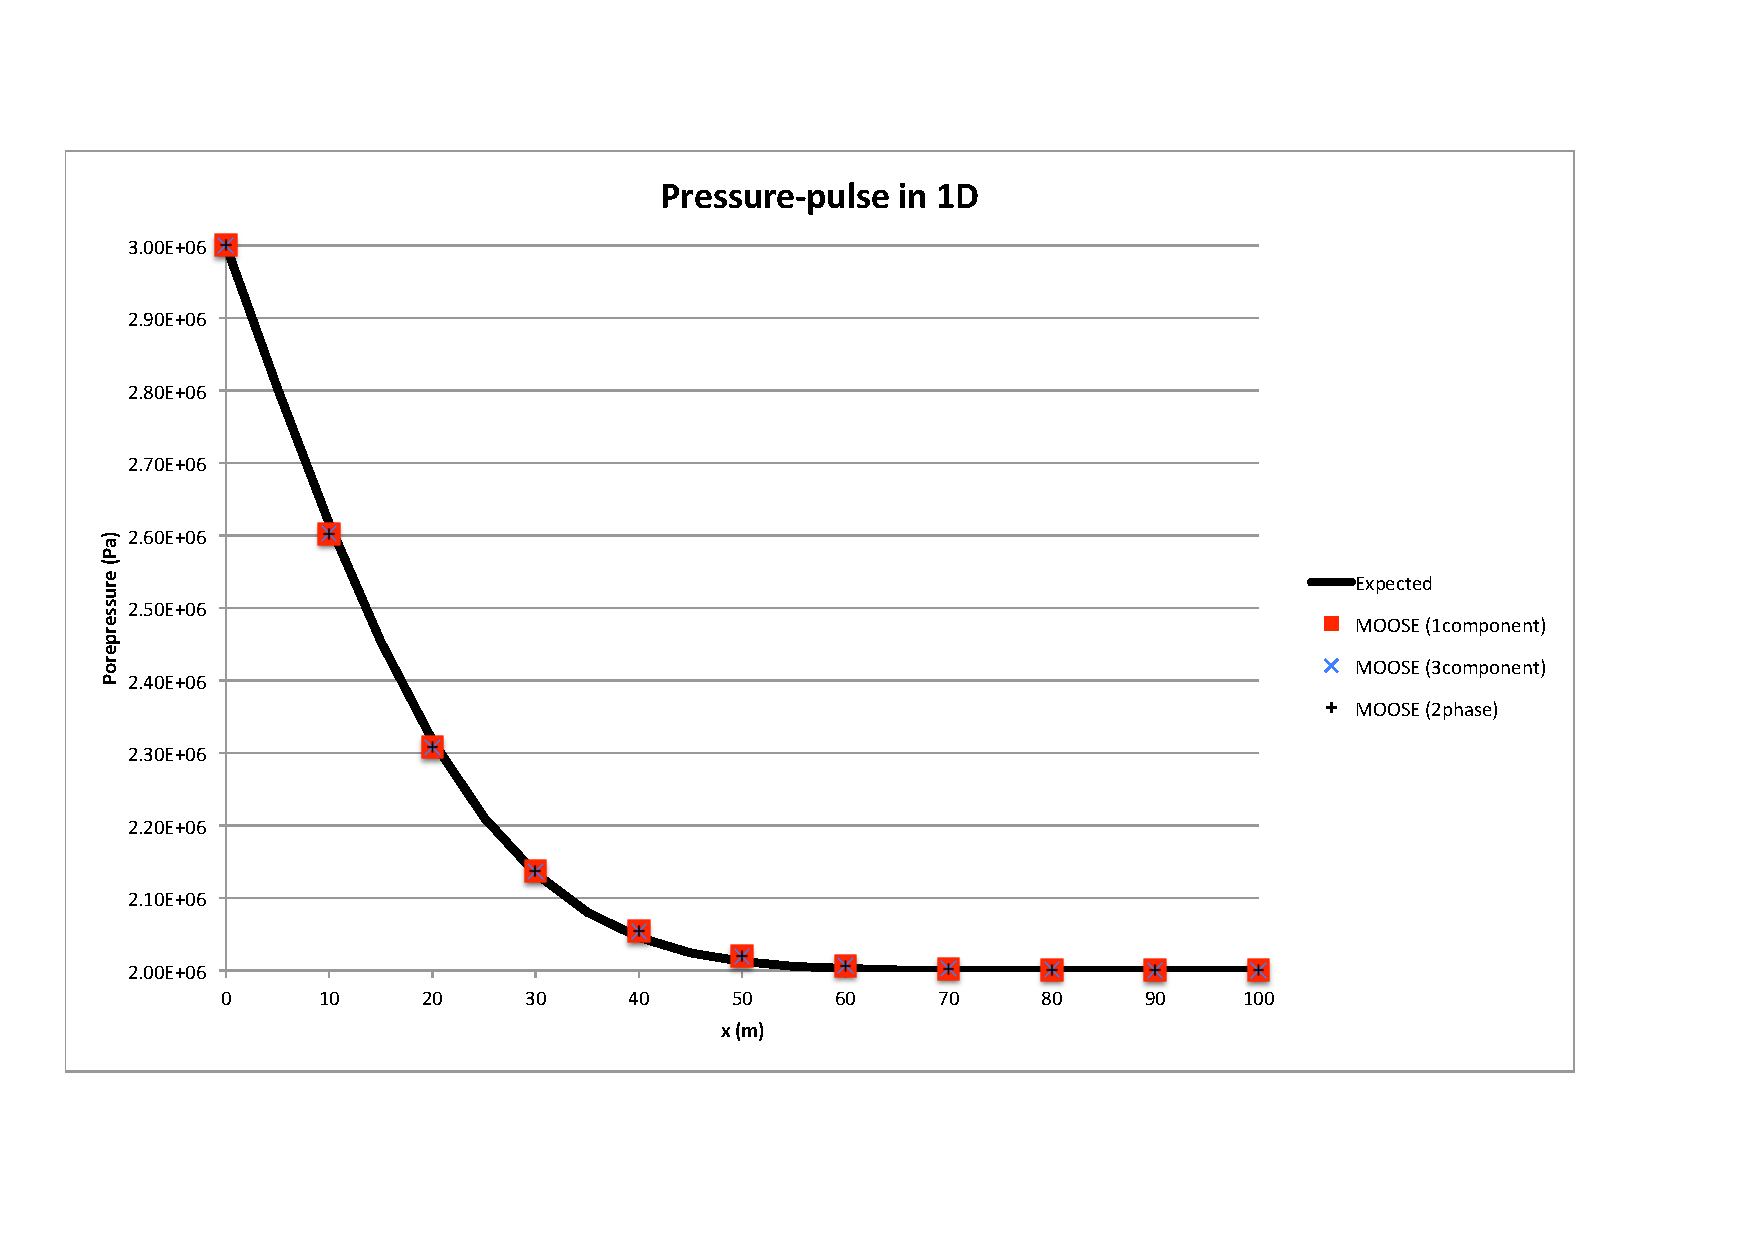
\includegraphics[width=15cm]{pressure_pulse_1d.pdf}
\caption{Comparison between the MOOSE result (in dots), and the
  exact analytic expression given by Eqn~(\ref{eqn.exact.pp}).  This
  test had 10 elements in the $x$ direction, with $0\leq x \leq
  100$\,m, and ran for a total of
  10$^4$ seconds with 10 timesteps.  The parameters were $B=2$\,GPa,
  $\kappa_{xx}=10^{-15}$\,m$^{2}$, $\mu=10^{-3}$\,Pa.s, $\phi=0.1$,
  with initial pressure $P=2$\,MPa, and applied pressure $P=3$\,MPa at
  $x=0$.  For greater spatial resolution and smaller timesteps the
  agreement increases.  Both the multi-component single-phase simulation and the
  2-phase fully-water-saturated simulation give identical results for
  the water porepressure.}
\label{pressure_pulse.fig}
\end{figure}



\end{document}


\chapter{Diffusion and dispersion}
\section{Diffusion}

The results of MOOSE are compared with the classical diffusion profile
for a simple 1D model with mass diffusion. In this example, the left end of
the mesh is held at a constant mass fraction of 1, while the right hand end is
prescribed a zero mass fraction boundary condition. No advection takes place, so
mass transfer is by diffusion only. This concentration profile has a well-known
similarity solution given by
\begin{equation}
C(u) = \erfc(u),
\end{equation}
where $\erfc(u)$ is the complentary error function, and $u = x/(2 \sqrt{D t})$ is the
similarity solution, $x$ is distance, $t$ is time, and $D$ is the diffusion coefficient.

The comparison between MOOSE and the analytical solution is presented in Figure \ref{fog:diff}, where we observe a very good agreement between the two solutions.
\begin{figure}[htb]
\centering
\includegraphics[width=12cm]{diffusion_fig.pdf}
\caption{Mass fraction profile from diffusion only}
\label{fig:diff}
\end{figure}

\section{Hydrodynamic dispersion}

The MOOSE results are compared to known analytical solutions for simple problems in order to vertify that the MOOSE implementation is working properly. For a simple 1D model with no diffusion and constant velocity $v$, an analytical solution for the mass fraction profile is given by Javendel et al. (1984)\footnote{Javandel, I, Doughty, C, Tsang, C-f, Groundwater Transport, Handbook of Mathematical Models, AGU, 1984},
\begin{align}
C(x, t) = & C_0 \left\{ \frac{1}{2} \erfc\left(\frac{x- v t}{2 \sqrt{D t}}\right) + \left(\frac{v^2 t}{\pi D}\right)^{1/2}
\exp \left(- \frac{\left[x - vt\right]^2}{4 D T}\right)\right. \nonumber \\
& - \left. \frac{1}{2} \left(1 + \frac{v x}{D} + \frac{v^2 t}{D} \right) \exp\left(\frac{v x}{D}\right) \erfc\left(\frac{x+v t}{2 \sqrt{D T}}\right)\right\},
\end{align}
where all parameters have been previously defined.

The comparison between the automatic test problem \emph{disp01} and the analytical solution is presented in Figure \ref{fig:disp}. The MOOSE results do not coincide with the analytical solution near the top and bottom of the concentration front due to numerical dispersion. If the number of elements in the mesh is increased and the time step size is reduced, numerical dispersion is reduced and a much closer fit to the analytical solution is obtained, see Figure \ref{fig:dispheavy}. This second test is marked as heavy as it takes approximately 5 seconds to run, but is available in the automatic test suite.
\begin{figure}[htb]
\centering
\includegraphics[width=12cm]{dispersion_fig.pdf}
\caption{Mass fraction profile from hydrodynamic dispersion only}
\label{fig:disp}
\end{figure}

\begin{figure}[htb]
\centering
\includegraphics[width=12cm]{dispersion_heavy_fig.pdf}
\caption{Mass fraction profile from hydrodynamic dispersion only using a more refined grid and smaller time steps}
\label{fig:dispheavy}
\end{figure}

\chapter{Infiltration problem}
\section{The 2-phase analytic infiltration solution}
\label{bw}

The physical setup studied in this section is a 1D column that is
initially unsaturated, and which is subject to a constant injection of
fluid from its top.  This is of physical importance because it is a
model of constant rainfall recharge to an initially dry groundwater system.
The top surface becomes saturated, and this saturated zone moves
downwards into the column, diffusing as it goes.  The problem is of
computational interest because under certain conditions an analytic
solution is available for the saturation profile as a function of
depth and time.

The Richards' equation for an incompressible fluid in one
spatial dimension ($z$) reads
\begin{equation}
\dot{S} = \nabla \left(D \nabla S\right) - \nabla K \ ,
\end{equation}
where
\begin{eqnarray}
D(S) & = & -\frac{\kappa \kappa_{rel}}{\mu\phi}P_{\mathrm{c}}' \ ,
\\
K(S) & = &\frac{\rho g \kappa\kappa_{\mathrm{rel}}}{\mu\phi} \ .
\end{eqnarray}
Here $P_{\mathrm{c}} = -P$ which is the capillary pressure, and recall
that $P_{\mathrm{c}}'(S)<0$.

The analytic solution of this nonlinear diffusion-advection relevant
to constant infiltration to groundwater has been derived Broadbridge
and White\footnote{P Broadbridge, I White ``Constant rate rainfall
  infiltration: A versatile nonlinear model, 1 Analytical solution''.
  Water Resources Research 24 (1988) 145--154.} for certain functions
$D$ and $K$.   Broadbridge and White
assume the hydraulic conductivity is
\begin{equation}
K(S) = K_{n} + (K_{s}-K_{n})\frac{\Theta^{2}(C-1)}{C-\Theta} \ ,
\label{bw.krel}
\end{equation}
where
\begin{equation}
\Theta = \frac{S - S_{n}}{S_{s} - S_{s}} \ ,
\end{equation}
and the parameters obey $0 \leq K_{n} < K_{s}$, $0 \leq S_{n} \leq S
\leq S_{s}\leq 1$, and $C>1$.  The diffusivity is of the form
$a(b-S)^{-2}$.  This leads to very complicated relationships between
the capillary pressure, $P_{c}$, and the saturation, except in the
case where $K_{n}$ is small, when they are related through
\begin{equation}
\frac{P_{\mathrm{c}}}{\lambda_{s}} = \frac{\Theta - 1}{\Theta} - \frac{1}{C}\log
\left( \frac{C-\Theta}{(C-1)\Theta} \right) \ ,
\end{equation}
with $\lambda_{s}>0$ being the final parameter introduced by
Broadbridge and White.

Broadbridge and White derive time-dependent solutions for constant
recharge to one end of a semi-infinite line.  Their solutions are
quite lengthy, so I will not write them here.  To compare with MOOSE,
I use the following parameters --- the hydraulic parameters are those
used in Figure~3 of Broadbridge and White:
\begin{center}
\begin{tabular}{|ll|}
\hline
Bar length & 20\,m \\
Bar porosity & 0.25 \\
Bar permeability & 1 \\
\hline
Gravity & 0.1\,m.s$^{-2}$ \\
\hline
Fluid density & 10\,kg.m$^{-3}$ \\
Fluid viscosity & 4\,Pa.s \\
\hline
$S_{n}$ & 0\,m.s$^{-1}$ \\
$S_{s}$ & 1\,m.s$^{-1}$ \\
$K_{n}$ & 0\,m.s$^{-1}$ \\
$K_{s}$ & 1\,m.s$^{-1}$ \\
$C$ & 1.5 \\
$\lambda_{s}$ & 2\,Pa \\
\hline
Recharge rate $R_{\ast}$ & 0.5 \\
\hline
\end{tabular} \\
\end{center}
Broadbridge and white consider the case where the initial condition is
$S=S_{s}$, but this yields $P=-\infty$, which is impossible to use in
a MOOSE model.  Therefore the initial condition $P=-900$\,Pa is used
which avoids any underflow problems.  The recharge rate of
$R_{\ast}=0.5$ corresponds in the MOOSE model to a recharge rate of
$0.5\rho\phi(\kappa_{s}-\kappa_{n})=1.25$\,kg.m$^{-2}$.s$^{-1}$.  Note
that I've chosen $\frac{\rho g \kappa}{\mu \phi} = 1$\,m.s$^{-1}$, so
that the $K_{n}$ and $K_{s}$ may be encoded as $\kappa_{n}=0$ and
$\kappa_{s}=1$ in the relative permeability function
Eqn~(\ref{bw.krel}) in a straightforward way.

Figure~\ref{bw.fig} shows good agreement between the analytic solution
of Broadbridge and White and the MOOSE implementation.  There are
minor discrepancies for small values of saturation: these get smaller
as the temporal and spatial resolution is increased, but never totally
disappear due to the initial condition of $P=-900$\,Pa.

Two tests are part of the automatic test suite (one is marked
``heavy'' because it is a high-resolution version).

\begin{figure}[htb]
\centering
\includegraphics[width=16cm]{bw.pdf}
\caption{Comparison of the Broadbridge and White analytical solution
  with the MOOSE solution for 3 times.  This figure is shown in the
  standard format used in the Broadbridge-White paper: the constant
  recharge is applied to the $\mbox{depth}=0$ surface, and gravity
  acts downwards in this figure.}
\label{bw.fig}
\end{figure}


\section{The two-phase analytic drainage solution}
\label{wli}

Warrick, Lomen and Islas\footnote{AW Warrick, DO Lomen and A Islas,
  ``An analytical solution to Richards' Equation for a Draining Soil
  Profile'', Water Resources Research 26 (1990) 253--258.} extended
the analysis of Broadbridge and White (Chapter~\ref{bw}) to include
the case of drainage from a medium.

The setup is an initially-saturated infinitely-long column of material
that drains freely from its lower end.  This is simulated by placing a
boundary condition of $P=0$ at the lower end.  To obtain their analytical
solutions, Warrick, Lomen and Islas make the same assumptions as
Broadbridge and White concerning the diffusivity and conductivity of
the medium.  Their solutions are quite lengthy, so I will not write
them here.

A MOOSE model with the parameters almost identical to those listed in
Chapter~\ref{bw} is compared with the analytical solutions.  The only
differences are that the ``bar'' length is 10000\,m (to avoid any
interference from the lower Dirichlet boundary condition), and
$R_{\ast}=0$ since there is no recharge.  The initial condition is
$P=10^{-4}$\,Pa: the choice $P=0$ leads to poor convergence since
by construction the Broadbridge-White capillary function is only
designed to simulate the unsaturated zone $P<0$ and a sensible
extension to $P\geq 0$ is discontinuous at $P=0$.

Figure~\ref{wli.fig} shows good agreement between the analytic
solution and the MOOSE implementation.  Any minor discrepancies get
smaller as the temporal and spatial resolution increase.

This test is part of the automatic test suite that is run every time
the code is updated.


\begin{figure}[htb]
\centering
\includegraphics[width=16cm]{wli.pdf}
\caption{Comparison of the Warrick, Lomen and Islas analytical solution
  with the MOOSE solution for 3 times.  This figure is shown in the
  standard format used in the literature: the top of the model is
  $\mbox{depth}=0$ surface, and gravity acts downwards in this figure,
with fluid draining from $\mbox{depth}=\infty$.}
\label{wli.fig}
\end{figure}



\chapter{Single-phase infiltration and drainage}
\label{forsyth}

Forsyth, Wu and Pruess\footnote{PA Forsyth, YS Wu and K Pruess,
  ``Robust numerical methods for saturated-unsaturated flow with dry
  initial conditions in heterogeneous media'', Advances in Water
  Resources 18 (1995) 25--38} describe a HYDRUS simulation of an
experiment involving infiltration (experiment 1) and subsequent
drainage (experiment 2) in a large caisson.  The simulation is
effectively one dimensional, and is shown in
Figure~\ref{rd_setup.fig}.

\begin{figure}[htb]
\begin{center}
\includegraphics[width=12cm]{rd_setup.eps}
\caption{Two experimental setups from Forsyth, Wu and Pruess.
  Experiment 1 involves infiltration of water into an initially
  unsaturated caisson.  Experiment 2 involves drainage of water from
  an initially saturated caisson.}
\label{rd_setup.fig}
\end{center}
\end{figure}

The properties common to each experiment
are:
\begin{center}
\begin{tabular}{|ll|}
\hline
Caisson & 0.33 \\
Caisson permeability & $2.95\times 10^{-13}$\,m$^{2}$ \\
\hline
Gravity & 10\,m.s$^{-2}$ \\
\hline
Water density & 1000\,kg.m$^{-3}$ \\
Water viscosity & 0.00101\,Pa.s \\
Water bulk modulus & 20\,MPa \\
Water residual saturation & 0.0 \\
Air residual saturation & 0.0 \\
Air pressure & 0.0 \\
\hline
van Genuchten $\alpha$ & $1.43\times 10^{-4}$\,Pa$^{-1}$ \\
van Genuchten $m$ & 0.336 \\
van Genuchten turnover & 0.99 \\
\hline
\end{tabular} \\
\end{center}
In each experiment 120 finite elements were used along the length of
the Caisson.  The modified van-Genuchten relative permeability curve
with a ``turnover'' (set at $S=0.99$) was employed in order to improve
convergence significantly.  Hydrus also uses a modified van-Genuchten
curve, although I couldn't find any details on the modification.

In experiment 1, the caisson is initially at saturation 0.303
($P=-72620.4$\,Pa), and water is pumped into the top with a rate
0.002315\,kg.m$^{-2}$.s$^{-1}$.  This causes a front of water to
advance down the caisson.  Figure~\ref{rd.result.fig} shows the
agreement between MOOSE and the published result (this result was
obtained by extracting data by hand from online graphics).

In experiment 2, the caisson is initially fully saturated at $P=0$,
and the bottom is held at $P=0$ to cause water to drain via the action
of gravity.  Figure~\ref{rd.result.fig} shows the agreement between
MOOSE and the published result.

Experiment 1 and the first 4 simulation days of experiment 2 are
marked as ``heavy'' in the PorousFlow test suite since the simulations
take around 3 seconds to complete.  This means they are not run by
default every time the code is updated, and must be run manually.
However, the final 96 days of experiment 2 run quickly and are part of
the automatic test suite.


\begin{figure}[htb]
\begin{center}
\includegraphics[width=12cm]{rd01.pdf} \\
$\mbox{}$\\
\includegraphics[width=12cm]{rd02.pdf}
\caption{Saturation profiles in the caisson.  Top: After 4.16 days of
  infiltration.  Bottom: After drainage from an initially-saturated
  simulation (4 days and 100 days profiles).  Note that the HYDRUS
  results are only approximate as I extrated the data by hand from
  online graphics.}
\label{rd.result.fig}
\end{center}
\end{figure}

\chapter{Water infiltration into a two-phase system}
\label{rsc}

An analytic solution of the two-phase Richards' equations with
gravity\footnote{Unfortunately there must be a typo in the RSC paper
  as for nonzero gravity their results are clearly incorrect.}  on a
semi-infinite line $z\geq 0$, with a constant water infiltration flux
at $z=0$ has been derived by Rogers, Stallybrass and
Clements\footnote{C Rogers, MP Stallybrass and DL Clements ``On two
  phase filtration under gravity and with boundary infiltration:
  application of a Backlund transformation'' Nonlinear Analysis,
  Theory, Methods and Applications 7 (1983) 785--799}.  The authors
assume incompressible fluids; linear relative permeability
relationships; the ``oil'' (or ``gas'') viscosity is larger than the
water viscosity; and, a certain functional form for the capillary
pressure.  When the oil viscosity is exactly twice the water
viscosity, their effective saturation reads
\begin{equation}
S_{\mathrm{eff}} = \frac{1}{\sqrt{1 + \exp((P_{c} - A)/B)}} \ ,
\label{eqn.rsc.seff}
\end{equation}
where $P_{c} = P_{\mathrm{oil}}-P_{\mathrm{water}}$ is the capillary
pressure, and $A$ and $B$ are arbitrary parameters to be defined by
the user in the MOOSE implementation.  For other oil/water viscosity
ratios $P_{c} = P_{c}(S_{\mathrm{eff}})$ is more complicated, and note
that their formulation allows $P_{c}<0$, but only
the particular form Eqn~(\ref{eqn.rsc.seff}) need be used to validate
the MOOSE implementation.

RSC's solutions are quite lengthy, so I will not write them here.  To
compare with MOOSE, the following parameters are used:
\begin{center}
\begin{tabular}{|ll|}
\hline
Bar length & 10\,m \\
Bar porosity & 0.25 \\
Bar permeability & $10^{-5}$\,m$^{2}$ \\
\hline
Gravity & 0\,m.s$^{-2}$ \\
\hline
Water density & 10\,kg.m$^{-3}$ \\
Water viscosity & $10^{-3}$\,Pa.s \\
\hline
Oil density & 20\,kg.m$^{-3}$ \\
Oil viscosity & $2\times 10^{-3}$\,Pa.s \\
\hline
Capillary $A$ & 10\,Pa \\
Capillary $B$ & 1\,Pa \\
\hline
Initial water pressure & 0\,Pa \\
Initial oil pressure & 15\,Pa \\
Initial water saturation & 0.08181 \\
Initial oil saturation & 0.91819 \\
\hline
Water injection rate & 1\,kg\,s$^{-1}$\,m$^{-2}$ \\
\hline
\end{tabular} \\
\end{center}

In the RSC theory water is injected into a semi-infinite domain,
whereas of course the MOOSE implementation has finite extent ($0\leq z
\leq 10$ is chosen).  Because of the near incompressibility of the
fluids (I choose the bulk modulus to be 2\,GPa) this causes the
porepressures to rise enormously, and the problem can suffer from
precision-loss problems.  Therefore, the porepressures are fixed at
$z=10$.  This does not affect the progress of the water saturation
front.  Figure~\ref{rsc.fig} shows good agreement between the analytic
solution and the MOOSE implementation.  Any minor discrepancies get
smaller as the temporal and spatial resolution increase, as is
suggested by the two comparisons in that figure.

The ``low-resolution'' test has 200 elements in $0\leq z\leq
10$ and uses 15 time steps is part the automatic test suite that
is run every time the code is updated.  The ``high-resolution'' test
has 600 elements and uses 190 time steps, and is marked as
``heavy''.

\begin{figure}[htb]
\begin{center}
\includegraphics[width=16cm]{rsc.pdf}
\caption{Water saturation profile for $t=5$\,s in the
  Rogers-Stallybrass-Clements test.  The initial water saturation is
  0.08181, and water is injected at the top of this figure at a
  constant rate.  This forms a water front which displaces the oil.
  Black line: RSC's analytic solution.  Red squares: high-resolution
  MOOSE simulation.  Green triangles: lower resolution MOOSE simulation.}
\label{rsc.fig}
\end{center}
\end{figure}

\include{buckley_leveret}
\chapter{Heat conduction}
\section{Simple heat conduction in 1D}

Porous-flow heat conduction is governed by the equation
\begin{equation}
0 = \frac{\partial}{\partial t}\energydens + \nabla\cdot \flux^{\mathrm{T}} \ ,
\label{eqn.heat.cond}
\end{equation}
Here $\energydens$ is the energy per unit volume in the rock-fluid
system, and $\flux^{\mathrm{T}}$ is the heat flux.  In the
porous-flow module
\begin{equation}
\energydens = (1 - \phi)\rho_{R}C_{R} T + \phi
\sum_{\phase}S_{\phase}\rho_{\phase}\energydens_{\phase} \ ,
\end{equation}
when there is no adsorbed species.  Here $T$ is the temperature,
$\phi$ is the rock porosity, and $S_{\phase}$ is the saturation of
phase $\phase$.  The remainder of the notation is described in the
next paragraph.  When studying problems involving heat conduction
(with no fluid convection)
\begin{equation}
\flux^{\mathrm{T}} = -\lambda\nabla T \ ,
\end{equation}
where $\lambda$ is the tensorial thermal conductivity of the
rock-fluid system.

The tests described in this section use the following simple forms for
each term
\begin{itemize}
\item $\rho_{R}$, which is the rock-grain density (that is, the
  density of rock with zero porespace), measured in kg.m$^{-3}$, is
  assumed constant in the current implementation of the PorousFlow
  module.
\item $C_{R}$, which is the rock-grain specific heat capacity, measured
  in J.kg$^{-1}$.K$^{-1}$, is assumed constant in the current
  implementation of the PorousFlow module.
\item $\rho_{\phase}$, which is the density of fluid phase $\phase$,
  is assumed in this chapter to be a function of the fluid pressure
  only (this is so Equation~(\ref{eqn.heat.cond}) may be easily solved
  --- more general forms are allowed in the PorousFlow module).
\item $\energydens_{\phase}$, which is the specific internal energy of the
  fluid phase $\phase$, and is measured in J.kg$^{-1}$, is assumed in
  this chapter to be
\begin{equation}
\energydens_{\phase} = C_{v}^{\phase} T \ ,
\end{equation}
where $C_{v}^{\phase}$ is the fluid's specific heat capacity at
constant volume.  This specific heat capacity is assumed constant (so
that Equation~(\ref{eqn.heat.cond}) may be easily solved --- more
general forms are allowed in the PorousFlow module).
\item $\lambda$ is assumed to vary between $\lambda^{\mathrm{dry}}$
  and $\lambda^{\mathrm{wet}}$, depending on the aqueous saturation:
\begin{equation}
\lambda_{ij} = \lambda_{ij}^{\mathrm{dry}} + S^{n} \left(
\lambda_{ij}^{\mathrm{wet}} - \lambda_{ij}^{\mathrm{dry}} \right) ,
\end{equation}
where $S$ is the aqueous saturation, and $n$ is a positive user-defined
exponent.  More general forms may be easily accommodated in the
PorousFlow module, but to date none have been coded.
\end{itemize}

Under these conditions, Equation~(\ref{eqn.heat.cond}) becomes
\begin{equation}
\dot{T} = \nabla_{i} \alpha_{ij} \nabla_{j} T \ .
\label{eqn.heat.cond.simple}
\end{equation}
The tensor $\alpha$ is
\begin{equation}
\alpha_{ij} = \frac{\lambda_{ij}}{(1 - \phi)\rho_{R}C_{R} +
  \rho\sum_{\phase}S_{\phase}\rho_{\phase}C_{v}^{\phase}} \ .
\end{equation}
For constant saturation and porepressure, $\alpha_{ij}$ is also constant.

Consider the one-dimensional case where the spatial dimension is the
semi-infinite line $x\geq 0$.  Suppose that initially the temperature is
constant, so that
\begin{equation}
T(x, t=0) = T_{0} \ \ \ \mbox{for }\ \ x\geq 0 \ .
\end{equation}
Then apply a fixed-pressure Dirichlet boundary condition at $x=0$ so
that
\begin{equation}
T(x=0, t>0) = T_{\infty}
\end{equation}
The solution of the above differential equation is well known to be
\begin{equation}
T(x, t) = T_{\infty} + (T_{0} -
T_{\infty})\,\mbox{Erf}\left( \frac{x}{\sqrt{4\alpha t}} \right) \ ,
\label{eqn.exact.pp}
\end{equation}
where Erf is the error function.

This is verified by using the following tests on a line of 10 elements.
\begin{enumerate}
\item A transient analysis with no fluids.  The parameters chosen are $\lambda_{ij} =
  \diag(2.2)$, $\phi=0.9$, $\rho_{R}=0.5$ and $C_{R}=2.2$ is chosen,
  so that $\alpha_{ij} = 1/(0.9\times 0.5)$.
\item A transient analysis with 2 fluid phases.  The parameters chosen
  are $\lambda^{\mathrm{dry}}=0.3$, $\lambda^{\mathrm{wet}} = 1.7$ and
  $S=0.5$, so that $\lambda_{ij} = \diag(1)$.  $\rho_{\mathrm{gas}} =
  0.4$, $\rho_{\mathrm{water}} = 0.3$, $\rho_{R}=0.25$, $C_{v}^{\mathrm{gas}} = 1$,
  $C_{v}^{\mathrm{water}}=2$, $C_{R}=1.0$, and $\phi=0.8$.  With these
  parameters, $\alpha_{ij} = 1/(0.9\times 0.5)$.
\end{enumerate}
An example verification is shown in Figure~\ref{heat_conduction.fig}.
These tests are part of the automatic test suite.

\begin{figure}[htb]
\centering
\includegraphics[width=15cm]{heat_conduction_1d.pdf}
\caption{Comparison between the MOOSE result (in dots), and the
  exact analytic expression given by Eqn~(\ref{eqn.exact.pp}).  This
  test had 10 elements in the $x$ direction, with $0\leq x \leq
  100$\,m, and ran for a total of
  10$^2$ seconds with 10 timesteps.}
\label{heat_conduction.fig}
\end{figure}

\chapter{Heat advection}
\section{One-dimensional heat advection via a single-phase fluid}

Consider the case of a single-phase fluid in 1 dimension, $0\leq x
\leq 1$, with the porepressure fixed at the boundaries:
\begin{equation}
P(x=0, t) = 1 \ \ \ \mbox{and}\ \ \ P(x=1, t) = 0 \ .
\end{equation}
With zero gravity, and high fluid bulk modulus, the Darcy equation
implies that the solution is $P(x, t) = 1 - x$, with
\begin{equation}
v = k/\mu
\end{equation}
being the constant\footnote{To get the velocity of the individual
  fluid particles, this should be divided by the porosity.} ``Darcy
velocity'' from $x=0$ to $x=1$.  Here $k$ is the porous medium's
permeability, and $\mu$ is the fluid dynamic viscosity.

Suppose that the fluid internal energy is given by $CT$, where $C$ is
the specific heat capacity and $T$ is its temperature.  Assuming that
$P/\rho \ll CT$, then the fluid's enthalpy is also $CT$.  In this
case, the energy equation reads
\begin{equation}
\left((1 - \phi)\rho_{R}C_{R} + \phi\rho C \right) \frac{\partial
  T}{\partial t} + C \rho v \frac{\partial T}{\partial x} = 0 \ .
\end{equation}
This is the wave equation with velocity
\begin{equation}
v_{T} = \frac{C\rho v}{(1 - \phi)\rho_{R}C_{R} + \phi\rho C} \ .
\end{equation}
Recall that the ``Darcy velocity'' is $v=k/\mu$.

Let the initial condition for $T$ be $T(x, t=0) = 200$.  Apply the
boundary conditions
\begin{equation}
T(x=0, t) = 300 \ \ \ \mbox{and} \ \ \ T(x=1, t) = 200 \ .
\end{equation}
At $t=0$ this creates a front at $x=0$.  Choose the parameters $C=2$,
$C_{R}=1$, $\rho=1000$, $\rho_{R}=125$, $\phi=0.2$, $k=1.1$, $\mu=4.4$
(all in consistent units), so that $v_{T}=1$ is the front's velocity.

The sharp front is {\em not} maintained by
MOOSE.  This is due to numerical diffusion, which is particularly
strong in the upwinding scheme implemented in the PorousFlow module.
Nevertheless, MOOSE advects the smooth front with the correct
velocity, as shown in Figure~\ref{heat_advection_1d.fig}.

The sharp front is {\em not} maintained by MOOSE even when no
upwinding is used.  In the case at hand, which uses a fully-saturated
single-phase fluid, the {\tt FullySaturated} versions of the Kernels
may be used in order to compare with the standard fully-upwinded
Kernels.  The {\tt FullySaturated} Kernels do not employ any upwinding
whatsoever, so less numerical
diffusion is expected.  This is demonstrated in
Figure~\ref{heat_advection_1d.fig}.  Two additional points may also be
nocied: (1) the lack of upwinding has produced a ``bump'' in the
temperature profile near the hotter side; (2) the lack of upwinding
means the temperature profile moves slightly slower than it should.
These two affects reduce as the mesh density is increased, however.

\begin{figure}[htb]
\begin{center}
\begin{tabular}{cc}
\includegraphics[width=7cm]{heat_advection_1d_0_1.pdf}  &
\includegraphics[width=7cm]{heat_advection_1d_0_6.pdf}
\end{tabular}
\caption{Results of heat advection via a fluid in 1D.  The fluid flows
  with constant Darcy velocity of $0.25$\,m.s$^{-1}$ to the right, and
  this advects a temperature front at velocity $1$\,m.s$^{-1}$ to the
  right.  The pictures above that the numerical implementation of
  porous flow within MOOSE (including upwinding) diffuses sharp
  fronts, but advects them at the correct velocity (notice the centre
  of the upwinded front is at the correct position in each picture).
  Less diffusion is experienced without upwinding.  Left: temperature
  $t=0.1$\,s.  Right: temperature at $t=0.6$\,s.}
\label{heat_advection_1d.fig}
\end{center}
\end{figure}

\chapter{Newton cooling}
\section{Classic Newton cooling in a bar}

Without fluids, mechanical deformation and sinks, the heat equation is
\begin{equation}
\rho_{R}C_{R}(1-\phi)\dot{T} = \nabla\lambda\nabla T \ ,
\end{equation}
where $\phi$ is the porosity, $\rho_{R}$ is the rock grain density
(kg.m$^{-3}$), $C_{R}$ is the rock grain specific heat capacity
(J.kg$^{-1}$.K$^{-1}$), $T$ is the temperature, and $\lambda$ is the
tensorial thermal conductivity of the porous material
(J.s$^{-1}$.K$^{-1}$.m$^{-1}$).

In section~\ref{pp.sec}, the dynamics of this equation is explored,
while this section concentrates on the steady-state situation.
Consider the one-dimensional case where a bar sits between $x=0$ and
$x=L$ with a fixed temperature at $x=0$:
\begin{equation}
T(x=0, t) = T_{0} \ ,
\end{equation}
and a sink flux at the other end:
\begin{equation}
\mbox{sink strength (J.m$^{-2}$.s$^{-1}$)} = \left.\lambda\frac{\partial
  T}{\partial x}\right|_{x=L} = -C\left(T - T_{e}\right)_{x=L} \ .
\label{eqn.heat.sink}
\end{equation}
Here $T_{e}$ is a fixed quantity (``e'' stands for ``external''), and
$C$ is a constant conductance (J.m$^{-2}$.s$^{-1}$.K$^{-1}$).

The solution is the linear function
\begin{equation}
T = T_{0} + \frac{T_{e} - T_{0}}{\lambda + C L} C x \ .
\end{equation}
The heat sink in Eqn~(\ref{eqn.heat.sink}) is a linear function of
$T$, so the {\tt PorousFlowPiecewiseLinearSink} may be employed.

The simulation is run in MOOSE using $C=1$, $L=100$, $\lambda=100$,
$T_{0}=2$ and $T_{e}=1$.  The solution is shown in Figure~\ref{nc_heat.fig}

\begin{figure}[htb]
\begin{center}
\includegraphics[width=16cm]{nc_temp.pdf}
\caption{The steady-state temperature in the bar.  MOOSE agrees well
  with theory illustrating that piecewise-linear heat sinks/sources
  and heat conduction are correctly implemented in MOOSE.}
\label{nc_heat.fig}
\end{center}
\end{figure}


\section{Porepressure sink in a bar}
\label{pp.sec}

These tests demonstrate that MOOSE behaves correctly when a simulation
contains a sink.  The sink is a piecewise linear function of pressure.

Darcy's equation for (single-phase) flow through a fully saturated medium without
gravity and without sources is
\begin{equation}
\frac{\partial}{\partial t}\phi\rho = \nabla_{i}\left(\frac{\rho
  \kappa_{ij}}{\mu} \nabla_{j}P \right) \ ,
\end{equation}
with the following notation:
\begin{itemize}
\item $\phi$ is the medium's porosity;
\item $\rho$ is the fluid density;
\item $\kappa_{ij}$ is the permeability tensor;
\item $\mu$ is the fluid viscosity;
\item $\partial/\partial t$ and $\nabla_{i}$ denote the time and spatial derivatives, respectively.
\end{itemize}
Using $\rho \propto
\exp(P/B)$, where $B$ is the fluid bulk modulus, Darcy's equation
becomes
\begin{equation}
\frac{\partial}{\partial t}\rho = \nabla_{i}\alpha_{ij}\nabla_{j}\rho \ ,
\end{equation}
with
\begin{equation}
\alpha_{ij} = \frac{\kappa_{ij}B}{\mu\phi} \ .
\end{equation}
Here the porosity and bulk modulus are assumed to be constant in space
and time.

Consider the one-dimensional case where a bar sits between $x=0$ and
$x=L$ with initial pressure distribution so $\rho(x,t=0) = \rho_{0}(x)$.
Maintain the end $x=0$ at constant pressure, so that $\rho(x=0, t) =
\rho_{0}(0)$.  At the end $x=L$, prescribe a sink flux
\begin{equation}
\left.\frac{\partial\rho}{\partial x}\right|_{x=L} = -C\left(\rho -
\rho_{e}\right)_{x=L} \ ,
\end{equation}
where $\rho_{e}$ is a fixed quantity (``e'' stands for ``external''),
and $C$ is a constant conductance.  This corresponds to the flux
\begin{equation}
\left.\frac{\partial P}{\partial x}\right|_{x=L} = -CB\left(1 -
e^{(P_{e}-P)/B}\right)_{x=L} \ ,
\end{equation}
which can easily be coded into a MOOSE input file: the flux is
$\rho\kappa\nabla P/\mu = -CB\kappa(e^{P/B} - e^{P_{e}/B})/\mu$, and
this may be represented by a piecewise linear function of pressure.

The solution of this problem is well known and is
\begin{equation}
\rho(x, t) = \rho_{0}(0) - \frac{\rho_{0}(0) - \rho_{e}}{1 + LC}Cx +
\sum_{n=1}^{\infty} a_{n}\sin \frac{k_{n}x}{L}e^{-k_{n}^{2}\alpha
  t/L^{2}} \ ,
\end{equation}
where $k_{n}$ is the $n^{\mathrm{th}}$ positive root of the equation
$LC\tan k + k=0$  ($k_{n}$ is a little bigger than
$(2n-1)\pi/2$), and $a_{n}$ is determined from
\begin{equation}
a_{n}\int_{0}^{L}\sin^{2}\frac{k_{n}x}{L}\,\mathrm{d}x =
\int_{0}^{L}\left(\rho_{0}(x) - \rho_{0}(0) + \frac{\rho_{0}(0) -
  \rho_{e}}{1 + LC}Cx\right)\sin \frac{k_{n}x}{L}\,\mathrm{d}x \ ,
\end{equation}
which may be solved numerically (Mathematica is used to generate
the solution in Figure~\ref{nc.fig}).

\noindent The problem is solved in MOOSE using the following parameters:
\begin{center}
\begin{tabular}{|ll|}
\hline
Bar length & 100\,m \\
Bar porosity & 0.1 \\
Bar permeability & $10^{-15}$\,m$^{2}$ \\
\hline
Gravity & 0 \\
\hline
Water density & 1000\,kg.m$^{-3}$ \\
Water viscosity & 0.001\,Pa.s \\
Water bulk modulus & 1\,MPa \\
\hline
Initial porepressure $P_{0}$ & 2\,MPa \\
Environmental pressure $P_{e}$ & 0 \\
\hline
Conductance $C$ & 0.05389\,m$^{-1}$ \\
\hline
\end{tabular} \\
\end{center}
This conductance is chosen so at steadystate $\rho(x=L)=2000$\,kg.m$^{-3}$.

The problem is solved using 1000 elements along the $x$ direction
($L=100$\,m), and using 100 time-steps of size $10^6$\,s.  Using fewer
elements or fewer timesteps means the agreement with the theory is
marginally poorer.  Two tests are performed: one with transient flow,
and one using the steadystate solver.  In this case the initial
condition is $P=2-x/L$\,MPa, since the uniform $P=2$\,MPa does not
converge.  The results are shown in Figure~\ref{nc.fig}.

\begin{figure}[htb]
\begin{center}
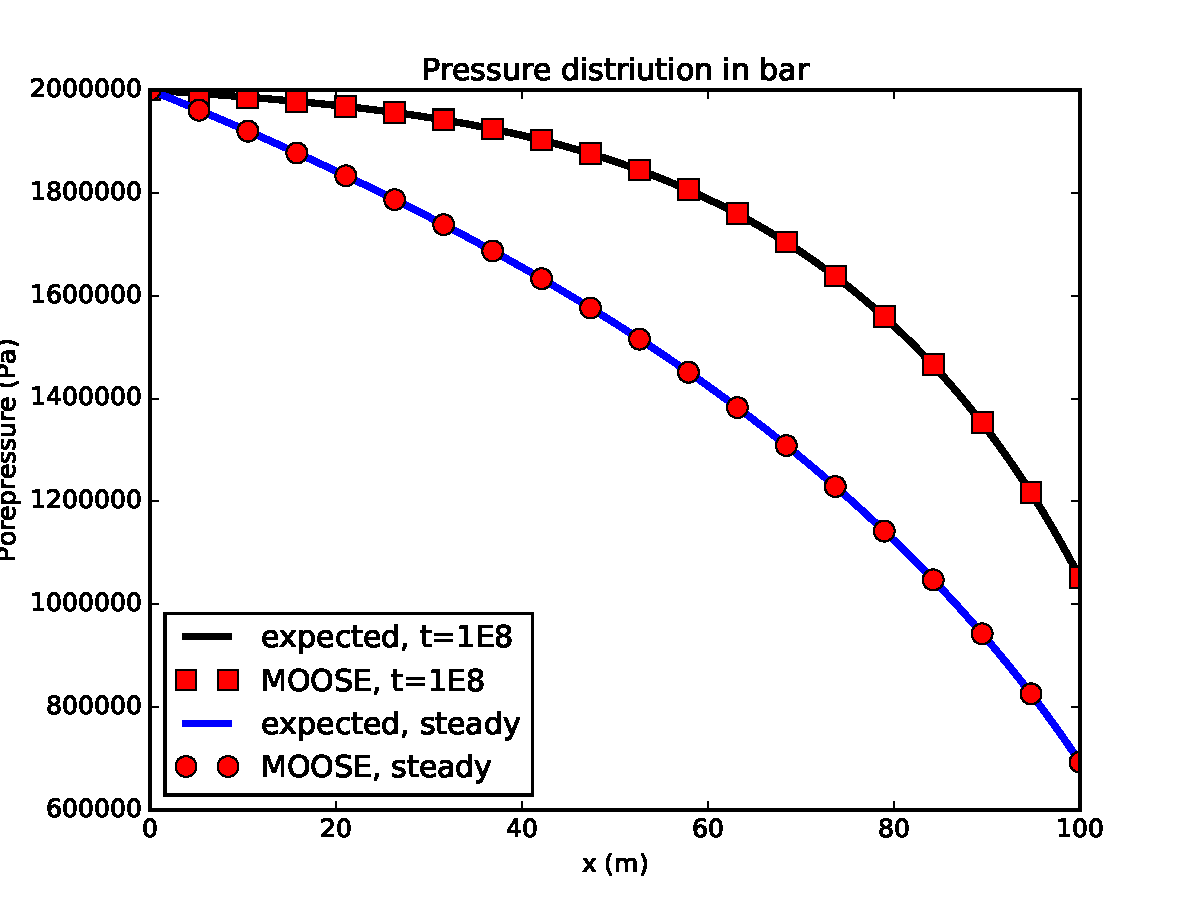
\includegraphics[width=17cm]{nc.pdf}
\caption{The porepressure in the bar at $t=10^{8}$\,s, and at
  steadystate.  The pressure at $x=0$ is held fixed, while the sink is
  applied at $x=100$\,m.  MOOSE agrees well with theory demonstrating
  that piecewise-linear sinks/sources and single-phase Darcy fluid
  flow are correctly implemented in MOOSE.}
\label{nc.fig}
\end{center}
\end{figure}


\section{Porepressure sink in a bar with heat}
\label{pp.heat.sec}

The simulation of Section~\ref{pp.sec} is re-run, but this time
heat flow is included.  In this section it is assumed that the fluid
specific enthalpy (J.kg$^{-1}$) is exactly equal to the fluid internal
energy, and that internal energy is ideal:
\begin{equation}
h = {\mathcal E} = C_{v}T \ .
\end{equation}
This makes the arguments below simple without having to consider real
fluids with complicated enthalpy and density expressions.

At the left end of the bar, the temperature is kept fixed:
\begin{equation}
T(x=0, t) = T_{0} \ .
\end{equation}
At the other end of the bar, heat is removed only by the fluid flowing
out of the system.  That is, there is a heat sink:
\begin{equation}
\mbox{sink strength (J.m$^{-2}$.s$^{-1}$)} = -C {\mathcal E}\left(\rho -
\rho_{e}\right)_{x=L} \ .
\end{equation}
No other sinks or sources are applied to the heat equation.

With this setup, the steady-state temperature in the bar must be
exactly
\begin{equation}
T(x, t=\infty) = T_{0} \ .
\end{equation}
For consider the fluid flowing from $x=0$ to $x=L$ in order to assume
steady-state.  At $x=0$ it must have temperature $T_{0}$ because that
temperature is fixed at $x=0$.  It advects this temperature with it as
it moves, so therefore at $t=\infty$, this temperature has permeated
throughout the entire bar.  This occurs even without heat conduction,
and is independent of the initial temperature of the bar.

MOOSE produces this result exactly.


\chapter{Hot ideal fluid in a bar}

This test uses a similar setup to Section~\ref{pp.heat.sec}, except
that here an ideal fluid is used.  The use of an ideal gas simplifies
the equations.  Only the steady-state is studied in this section.

The governing equation for the fluid's porepressure $P$ is
\begin{equation}
\nabla \frac{\rho\kappa}{\mu}\nabla P = 0 \ .
\end{equation}
It is assumed that $\kappa$ and $\mu$ are constant, and that
\begin{equation}
\rho = \frac{MP}{RT} \ ,
\end{equation}
holds (this is the ideal gas equation of state).  In this formula $M$
is the gas molar mass, $R$ is the gas constant and $T$ is the
temperature.

The equation governing the temperature is assumed to be just the fluid
advection equation
\begin{equation}
\nabla\frac{h\rho\kappa}{\mu}\nabla P = 0 \ .
\end{equation}
As in Section~\ref{pp.heat.sec}, heat conduction could be added, but
it is actually irrelevant since the solution to the problem below is
constant $T$.  The enthalpy, $h$, for an ideal gas is
\begin{equation}
h = C_{v}T + \frac{P}{\rho} = C_{v}T + \frac{RT}{M} = C_{p}T \ .
\end{equation}

The boundary conditions at the left-hand end are
\begin{equation}
P(x=0) = P_{0} \ \ \ \mbox{and}\ \ \ T(x=0)=T_{0} \ .
\end{equation}
Physically these correspond to fluid and heat being removed or added
to the left-hand end by some external source in order to keep the
porepressure and temperature fixed.

The porepressure boundary condition
at the right-hand end of the bar is
\begin{equation}
\mbox{sink flux (kg.m$^{-2}$.s$^{-1}$)} =
\left. \frac{\rho\kappa}{\mu}\nabla P \right|_{x=L} =
\left. -C\frac{\rho\kappa}{\mu} (P - P_{e}) \right|_{x=L} \ .
\label{ideal.mass.bdy}
\end{equation}
Physically this corresponds to the mass-flow through the boundary
being proportional to $P-P_{e}$.  Here $P_{e}$ is a fixed
``environmental'' porepressure, and this acts as a source or sink of
fluid.  $C$ is the ``conductance'' of the boundary.  Notice the
appearence of $\rho \kappa/\mu$ in the LHS of this equation means that
this is truly a flux of fluid mass (measured in kg.m$^{-2}$.s$^{-1}$),
and the appearence of $\rho\kappa/\mu$ on the RHS means that a {\tt
  PorousFlowPiecewiseLinearFlux} may be used with {\tt
  use\_mobility=true}.

The temperature boundary condition
at the right-hand end of the bar is
\begin{equation}
\mbox{heat flux (J.m$^{-2}$.s$^{-1}$)} =
\left. \frac{h\rho\kappa}{\mu}\nabla P \right|_{x=L} =
\left. -C\frac{h\rho\kappa}{\mu} (P - P_{e}) \right|_{x=L} \ .
\end{equation}
Comparing this with Equation~\ref{ideal.mass.bdy}, it is seen that
this is exactly the heat loss (or gain) at the boundary corresponding
to the loss (or gain) of the fluid.  Notice the appearence of $h\rho
\kappa/\mu$ in the LHS of this equation means that this is truly a
flux of fluid mass (measured in J.m$^{-2}$.s$^{-1}$), and the
appearence of $h\rho\kappa/\mu$ on the RHS means that a {\tt
  PorousFlowPiecewiseLinearFlux} may be used with {\tt
  use\_mobility=true} and {\tt use\_enthalpy=true}.

There is a clear similarity between the fluid and heat equations.  The
heat equation does not actually depend on temperature, and is simply
\begin{equation}
0 = \nabla (P\nabla P) \ ,
\end{equation}
which is solved by
\begin{equation}
P^{2} = P_{0}^{2} + Ax \ .
\end{equation}
The fluid equation then yields
\begin{equation}
T(x) = T_{0} \ .
\end{equation}
The constant $A$ may be determined from the either of the boundary
conditions.  For the special case of $P_{e}=0$ and $2LC=1$, the
solution is
\begin{equation}
P = P_{0} \sqrt{1 - \frac{x}{2L}} \ .
\end{equation}
MOOSE produces this result exactly, as illustrated in Figure~\ref{nc08.fig}

\begin{figure}[htb]
\begin{center}
\includegraphics[width=17cm]{nc08.pdf}
\caption{The steady-state porepressure and temperature distributions
  in the bar ($P_{0}=200$ and $T_{0}=180$).  MOOSE agrees well with
  theory illustrating that piecewise-linear fluid and heat
  sinks/sources as well as ideal fluids are correctly implemented in
  MOOSE.}
\label{nc08.fig}
\end{center}
\end{figure}

\chapter{Poroelasticitiy}
\section{Introduction}

The PorousFlow module includes the ability to couple fluid flow to
solid mechanics, and thus includes poroelasticity, which is the theory
of a fully-saturated single-phase fluid with constant bulk density and
constant viscosity coupled to small-strain isotropic elasticity.

There is one important difference between the theories, however.  The
time-derivative terms of poroelasticity are
\begin{equation}
\frac{1}{M}\dot{P} + \alpha\dot{\epsilon}_{ii} \ ,
\label{eqn.poro.dt}
\end{equation}
where $M$ is the Biot modulus:
\begin{equation}
\frac{1}{M} = \frac{(1-\alpha)(\alpha - \phi)}{K} +
\frac{\phi}{K_{\mathrm{f}}} \ ,
\label{biotmod.eqn}
\end{equation}
$P$ is the fluid porepressure, $\alpha$ is the Biot coefficient,
$\epsilon_{ii}$ is the volumetric strain, $\phi$ is the porosity, $K$
is the solid (drained) bulk modulus, and $K_{\mathrm{f}}$ is the fluid
bulk modulus.  Evidently from Eqn~(\ref{biotmod.eqn}), the Biot
modulus, $M$, should evolve with time as the porosity evolves.
Indeed, the terms in Eqn~(\ref{eqn.poro.dt}) are derived from the
continuity equation $\partial (\phi\rho)/\partial t +
\phi\rho\dot{\epsilon}_{ii}$ using the evolution of $\phi$ (and that
$\rho = \rho_{0}\exp(P/K_{\mathrm{f}})$).  However, in the standard
analytical solutions of poroelasticity theory, the Biot modulus, $M$
is considered fixed.

The PorousFlow module allows porosity to vary with fluid porepressure
and volumetric strain, so usually the Biot modulus would vary too,
causing differences with the analytical solutions of poroelasticity.
Therefore, PorousFlow offers a porosity relationship that evolves
porosity in such a way as to keep $M$ fixed.  This is called {\tt
  PorousFlowPorosityHMBiotModulus}.

PorousFlow is also built with finite strains in mind, whereas
poroelasticity is not.  Therefore, in comparisons with solutions from
poroelasticity theory, either the strain should be kept small, or the
various finite-strain switches in PorousFlow should be turned off
(they are all on by default).

\section{Volumetric expansion due to increasing porepressure}

The porepressure within a fully-saturated sample is increased:
\begin{equation}
P_{\mathrm{f}} = t \ .
\end{equation}
Zero mechanical pressure is applied to the sample's exterior, so that
no Neumann BCs are needed on the sample.  No fluid flow occurs since
the porepressure is increased uniformly throughout the sample

The effective stresses should then evolve as
$\sigma_{ij}^{\mathrm{eff}} = \alpha t \delta_{ij}$, and the
volumetric strain $\epsilon_{00}+\epsilon_{11}+\epsilon_{22} = \alpha
t/K$.  MOOSE produces this result correctly.

\section{Undrained oedometer test}

A cubic single-element fully-saturated sample has roller BCs applied
to its sides and bottom.  All the sample's boundaries are impermeable.
A downwards (normal) displacement, $u_{z}$, is applied to its
top, and the rise in porepressure and effective stress is observed.
(Here $z$ denotes the direction normal to the top face.)  There is
no fluid flow in the single element.

Under these conditions, assuming constant porosity, and denoting the
height ($z$ length) of the sample by $L$:
\begin{eqnarray}
P_{\mathrm{f}} & = & -K_{f}\log(1 - u_{z}) \ , \nonumber \\
\sigma_{xx}^{\mathrm{eff}} & = & (K - \mbox{$\frac{2}{3}$}G)u_{z}/L \ , \nonumber \\
\sigma_{zz}^{\mathrm{eff}} & = & (K + \mbox{$\frac{4}{3}$}G)u_{z}/L \ .
\end{eqnarray}

\section{Porepressure generation of a confined sample}

A single-element fully-saturated sample is constrained on all sides
and its boundaries are impermeable.  Fluid is pumped into the sample
via a source $s$ (kg.s$^{-1}$.m$^{-3}$) and the rise
in porepressure is observed.

Denoting the strength of the source by $s$ (units are s$^{-1}$), the expected result is
\begin{eqnarray}
\mbox{fluid mass} & = & \mbox{fluid mass}_{0} + st \ , \nonumber \\
\sigma_{ij}^{\mathrm{eff}} & = & 0 \ , \nonumber \\
P_{\mathrm{f}} & = & K_{\mathrm{f}}\log(\rho\phi/\rho_{0}) \ , \nonumber
\\
\rho & = & \rho_{0}\exp(P_{\mathrm{f}}/K_{f}) \ , \nonumber \\
\phi & = & \alpha + (\phi_{0}-\alpha)\exp\left(
P_{\mathrm{f}}(\alpha - 1)/K\right) \ . \\
\end{eqnarray}
Here $K$ is the solid bulk modulus.

\section{Porepressure generation of an unconfined sample}

A single-element fully-saturated sample is constrained on all sides,
except its top.  All its boundaries are impermeable.  Fluid is pumped
into the sample via a source $s$ (kg.s$^{-1}$.m$^{-3}$)) and the rise
in the top surface, the porepressure, and the stress are observed.

Regardless of the evolution of porosity, the following ratios result
\begin{eqnarray}
\sigma_{xx}/\epsilon_{zz} & = & K - 2G/3 \ , \nonumber \\
\sigma_{zz}/\epsilon_{zz} & = & K + 4G/3 \ , \nonumber \\
P/\epsilon_{zz} & = & (K + 3G/3 + \alpha^{2}M)/\alpha - \alpha M \ .
\end{eqnarray}
where $K$ is the undrained bulk modulus, $G$ the shear modulus,
$\alpha$ the Biot coefficient, and $M$ is the initial Biot modulus.
MOOSE produces these results when using the {\tt
  PorousFlowPorosityHM} material.


However, if the Biot modulus, $M$, is held fixed as the porosity
evolves, and the source is
\begin{equation}
s = S \rho_{0}\exp(P/K_{\mathrm{f}}) \ ,
\end{equation}
with $S$ being a {\em constant} volumetric source
(m$^{3}$.s$^{-1}$.m$^{-3}$) then
\begin{eqnarray}
\epsilon_{zz} & = & \frac{\alpha M s t}{K + 4G/3 + \alpha^{2}M} \ ,
\nonumber \\
P & = & M(st - \alpha\epsilon_{zz}) \ , \nonumber \\
\sigma_{xx} & = & (K - 2G/3)\epsilon_{zz} \ , \nonumber \\
\sigma_{zz} & = & (K + 4G/3)\epsilon_{zz} \ .
\end{eqnarray}
MOOSE produces these results when using the {\tt
  PorousFlowPorosityHMBiotModulus} material.

\section{Terzaghi consolidation}

This is documented at {\tt
  http://mooseframework.org/wiki/PhysicsModules/TensorMechanics/TensorMechanicsBasics/PoroMechanics/}.
The PorousFlow Material {\tt PorousFlowPorosityHMBiotModulus} must be used.

\section{Mandel's consolidation of a drained medium}

A sample's dimensions are $-a \leq x \leq a$ and $-b \leq y \leq b$,
and it is in plane strain (no $z$ displacement).  It is squashed with
constant normal force by impermeable, frictionless plattens on its top
and bottom surfaces (at $y = \pm b$).  Fluid is allowed to leak out
from its sides (at $x = \pm a$), but all other surfaces are
impermeable.  This is called Mandel's problem and it is shown
graphically in Fig~\ref{mandel_setup.fig}

\begin{figure}[htb]
\begin{center}
\includegraphics[width=8cm]{mandel_setup.pdf}
\caption{The setup of the Mandel experiment: a force $F$ squashes a
  porous material with impermeable plattens.  This causes fluid to
  seep from the material.}
\label{mandel_setup.fig}
\end{center}
\end{figure}

The interesting feature of this problem (apart from that it can be
solved analytically) is that the porepressure in the sample's center
actually increases for a short time after application of the force.
This is because the leakage of the fluid from the sample's sides
causes an apparent softening of the material near those sides.  This
means stress concentrates towards the sample's center which causes an
increase in porepressure.  Of course, eventually the fluid totally
drains from the sample, and the porepressure is zero.  As the fluid
drains from the sample's sides the plattens move slowly towards each
other.

The solution for porepressure and displacements is given in: AHD Cheng
and E Detournay ``A direct boundary element method for plane strain
poroelasticity'' International Journal of Numerical and Analytical
Methods in Geomechanics 12 (1988) 551-572.  The solution involves
rather lengthy infinite series, so I will not write it here.

As is common in the literature, this is simulated by considering the
quarter-sample, $0\leq x \leq a$ and $0\leq y\leq b$, with
impermeable, roller BCs at $x=0$ and $y=0$ and $y=b$.  Porepressure is
fixed at zero on $x=a$.  Porepressure and displacement are initialised
to zero.  Then the top ($y=b$) is moved downwards with prescribed
velocity, so that the total force that is induced by this downwards
velocity is fixed.  The velocity is worked out by solving Mandel's
problem analytically, and the total force is monitored in the
simulation to check that it indeed remains constant.

The simulations in the PorousFlow test suite use 10 elements in the
$x$ direction and 1 in the $y$ direction.  Four types of simulation
are run:
\begin{enumerate}
\item HM.  This uses standard PorousFlow Materials and Kernels, in
  particular it uses the ``HM'' porosity relationship.  This is not
  expected to agree perfectly with the analytical solutions because:
  the solutions assume constant Biot modulus.
\item constM.  This is identical to the HM case, save that it uses a
  porosity evolution law that keeps the Biot modulus fixed.  It is
  therefore expected to agree with the analytical solutions.
\item FullSat.  This uses the FullySaturated versions of the fluid
  mass time derivative and the fluid flux.  In this case the Biot
  modulus is kept fixed, so it is expected to agree with the
  analytical solutions.
\item FullSatVol.  This uses the FullySaturated versions of the fluid
  mass time derivative and the fluid flux, and does not multiply by
  the fluid density.  Therefore this version is identical to what is
  usually implemented in poro-elastic codes.  It is linear and
  therefore converges in only one iteration.  In this case the Biot
  modulus is kept fixed, so it is expected to agree with the
  analytical solutions.
\end{enumerate}
Of course there are minor discrepancies between the last three and the
analytical solution that are brought about through spatial and
temporal discretisation errors.  The figures below present the
results.

\begin{figure}[htb]
\begin{center}
\includegraphics[width=11cm]{mandel_ver_disp.pdf}
\caption{The vertical displacement of the platten as a function of time.}
\label{mandel_ver_disp.fig}
\end{center}
\end{figure}

\begin{figure}[htb]
\begin{center}
\includegraphics[width=11cm]{mandel_hor_disp.pdf}
\caption{The horizontal displacement of the material at $(x,y) = (a,
  b)$ as a function of time.}
\label{mandel_hor_disp.fig}
\end{center}
\end{figure}


\begin{figure}[htb]
\begin{center}
\includegraphics[width=11cm]{mandel_HM.pdf}
\caption{The porepressure at various points in the sample in the HM
  model with $a=1$.}
\label{mandel_HM.fig}
\end{center}
\end{figure}


\begin{figure}[htb]
\begin{center}
\includegraphics[width=11cm]{mandel_FSV.pdf}
\caption{The porepressure at various points in the sample in the FullSatVol
  model with $a=1$.}
\label{mandel_FSV.fig}
\end{center}
\end{figure}

\begin{figure}[htb]
\begin{center}
\includegraphics[width=11cm]{mandel_force.pdf}
\caption{The total downwards force on the platten as a function of
  time.  This should be unity.}
\label{mandel_force.fig}
\end{center}
\end{figure}

\chapter{Plastic Heat}
\section{Plastic deformation heating a porous skeleton}

In this section, plastic deformation causes a heat energy-density rate
(J.m$^{-3}$.s$^{-1}$) of
\begin{equation}
c (1-\phi) \sigma_{ij}\epsilon^{\mathrm{plastic}}_{ij} \ ,
\end{equation}
where $c$ is a coefficient (s$^{-1}$), $\phi$ is the porosity,
$\sigma$ is the stress, and $\epsilon^{\mathrm{plastic}}$ is the
plastic strain.

There is no fluid, and no heat flow is studied: the heat energy
released simply heats up the porous skeleton:
\begin{equation}
\frac{\partial}{\partial t} (1 - \phi)c_{R}\rho_{R} T = c (1-\phi)
\sigma_{ij}\epsilon^{\mathrm{plastic}}_{ij} \ .
\end{equation}
The porosity ($\phi$) and volumetric heat
capacity of the rock grains ($c_{R}\rho_{R}$) are chosen to be constant.

Perfect capped weak-plane plasticity is used, so that the admissible
zone is defined by
\begin{eqnarray}
\sigma_{zz} & \leq & S_{T} \ , \\
\sigma_{zz} & \geq & -S_{C} \, \\
\sqrt{\sigma_{zx}^{2} + \sigma_{zy}^{2}} + \sigma_{zz}\tan\Phi & \leq
& C \ .
\end{eqnarray}
Here $S_{T}$ is the tensile strength, $S_{C}$ is the compressive
strength, $C$ is the cohesion and $\Phi$ is the friction angle.  The
elastic tensor is chosen to be
\begin{equation}
E_{ijkl} = \lambda \delta_{ij}\delta_{kl} + \mu
(\delta_{ik}\delta_{jl} + \delta_{il}\delta_{jk}) \ .
\end{equation}
The parameters in these expressions are chosen to be: $S_{T}=1$,
$S_{C}=1$, $C=1$, $\Phi=\pi/4$, $\lambda=1/2$, and $\mu=1/4$ (all in
consistent units).

In each experiment a single finite-element is used.

\section{Tensile failure}

The top of the finite element is pulled upwards with displacement:
\begin{equation}
u_{z} = zt \ ,
\end{equation}
while the displacement in the $x$ and $y$ directions is chosen to be
zero.  This implies the only non-zero component of total strain is
\begin{equation}
\epsilon^{\mathrm{total}}_{zz} = t \ .
\end{equation}
The constitutive law implies
\begin{equation}
\sigma_{zz} = t \ .
\end{equation}
This stress is admissible for $t\leq 1$, while for $t>1$ the system
yields in tension:
\begin{equation}
\sigma_{zz} = 1 \ \ \ \mbox{for } t>1 \ ,
\end{equation}
and the plastic strain is,
\begin{equation}
\epsilon^{\mathrm{plastic}}_{zz} = t - 1 \ \ \ \mbox{for } t>1 \ .
\end{equation}
This means that the material's temperature should increase as
\begin{equation}
c_{R}\rho_{R}\dot{T} = c \ \ \ \mbox{for } t>1 \ ,
\end{equation}
while the right-hand side is zero for $t\leq 1$.

\section{Compressive failure}

The top of the finite element is pushed downwards with displacement:
\begin{equation}
u_{z} = -zt \ ,
\end{equation}
while the displacement in the $x$ and $y$ directions is chosen to be
zero.  This implies only non-zero component of total strain is
\begin{equation}
\epsilon^{\mathrm{total}}_{zz} = -t \ .
\end{equation}
The constitutive law implies
\begin{equation}
\sigma_{zz} = -t \ .
\end{equation}
This stress is admissible for $t\leq 1$, while for $t>1$ the system
yields in compression
\begin{equation}
\sigma_{zz} = -1 \ \ \ \mbox{for } t>1 \ ,
\end{equation}
and the plastic strain is,
\begin{equation}
\epsilon^{\mathrm{plastic}}_{zz} = -(t - 1) \ \ \ \mbox{for } t>1 \ .
\end{equation}
This means that the material's temperature should increase as
\begin{equation}
c_{R}\rho_{R}\dot{T} = c \ \ \ \mbox{for } t>1 \ ,
\end{equation}
while the right-hand side is zero for $t\leq 1$.

\section{Shear failure}

The top of the finite element is sheared with displacement:
\begin{equation}
u_{x} = zt \ ,
\end{equation}
while the displacement in the $y$ and $z$ directions is chosen to be
zero.  This implies only non-zero component of total strain is
\begin{equation}
\epsilon^{\mathrm{total}}_{xz} = t \ .
\end{equation}
The constitutive law implies
\begin{equation}
\sigma_{xz} = t/4 \ .
\end{equation}
This stress is admissible for $t\leq 4$, while for $t>4$ the system
yields in shear:
\begin{equation}
\sigma_{xz} = 1 \ \ \ \mbox{for } t>4 \ ,
\end{equation}
and the plastic strain is,
\begin{equation}
\epsilon^{\mathrm{plastic}}_{xz} = t - 4 \ \ \ \mbox{for } t>4 \ .
\end{equation}
This means that the material's temperature should increase as
\begin{equation}
c_{R}\rho_{R}\dot{T} = c \ \ \ \mbox{for } t>4 \ ,
\end{equation}
while the right-hand side is zero for $t\leq 4$.


\end{document}
